\documentclass[12pt,a4paper]{article}

% ------------------------------------------------------------
% Fonts & layout
% ------------------------------------------------------------
\usepackage[T1]{fontenc}
\usepackage[utf8]{inputenc}
\usepackage{lmodern}
\usepackage{microtype}
\usepackage{geometry}
\geometry{margin=1in}
\usepackage{array}
\usepackage{booktabs}

% ------------------------------------------------------------
% Math
% ------------------------------------------------------------
\usepackage{amsmath,amssymb,amsthm,mathtools}

% Standard operators
\DeclareMathOperator{\id}{id}
\DeclareMathOperator{\im}{im}
\DeclareMathOperator{\coker}{coker}
\DeclareMathOperator{\Hom}{Hom}

\DeclareMathOperator{\Spec}{Spec}
\DeclareMathOperator{\Proj}{Proj}

% Categories / notation
\newcommand{\Ab}{\mathbf{Ab}}
\newcommand{\PreSh}{\mathbf{PreSh}}
\newcommand{\Sh}{\mathbf{Sh}}

\newcommand{\F}{\mathcal F}


% basic number sets
\newcommand{\RR}{\mathbb{R}}

% sheaf letters

\newcommand{\G}{\mathcal G}

\newcommand{\GG}{\mathbb G}


\newcommand{\AffSch}{\mathbf{AffSch}}
\newcommand{\ZZ}{\mathbb Z}

\newcommand{\PP}{\mathbb P}

\usepackage{tikz}
\usetikzlibrary{decorations.pathreplacing}
\usetikzlibrary{positioning,arrows.meta}

% sheaf of continuous real-valued functions
\newcommand{\Czero}{\mathcal C^0}        % “C^0”
\newcommand{\CzeroX}{\mathcal C^0_X}     % sheaf on X (optional)

\newcommand{\Cinfty}{\mathcal C^\infty}
\newcommand{\CinftyM}{\mathcal C^\infty_M} % if you use C^\infty_M

% number sets / standard symbols
\newcommand{\CC}{\mathbb{C}}

% structure sheaf notation in complex geometry
\newcommand{\OO}{\mathcal{O}}
\newcommand{\OOX}{\mathcal{O}_X} % optional convenience



\newcommand{\Sch}{\mathrm{Sch}}
\newcommand{\Rings}{\mathrm{Rings}}

\newcommand{\kappares}{\kappa}
\newcommand{\GammaX}{\Gamma(X,\mathcal O_X)}

\newtheorem{theorem}{Theorem}[section]
\newtheorem{proposition}[theorem]{Proposition}
\newtheorem{lemma}[theorem]{Lemma}

\newcommand{\nilrad}{\sqrt{(0)}}

\newcommand{\Frac}{\operatorname{Frac}}


\providecommand{\Spec}{\operatorname{Spec}}
\providecommand{\A}{\mathbb A}
\providecommand{\Pj}{\mathbb P}
\providecommand{\G}{\mathbb G}

% ------------------------------------------------------------
% Links
% ------------------------------------------------------------
\usepackage{xcolor}
\usepackage{hyperref}
\usepackage{bookmark}
\hypersetup{
  colorlinks=true,
  linkcolor=blue!50!black,
  urlcolor=blue!50!black,
  citecolor=blue!50!black,
  pdftitle={Algebraic Geometry 5
  },
  pdfauthor={},
  pdfsubject={Lecture notes (reorganized)},
  pdfcreator={TeXStudio / LaTeX}
}

% ------------------------------------------------------------
% Diagrams
% ------------------------------------------------------------
\usepackage{tikz-cd}

% ------------------------------------------------------------
% Lists
% ------------------------------------------------------------
\usepackage{enumitem}
\setlist[itemize]{topsep=4pt,itemsep=2pt,parsep=0pt,partopsep=0pt}
\setlist[enumerate]{topsep=4pt,itemsep=2pt,parsep=0pt,partopsep=0pt}

% ------------------------------------------------------------
% Theorem environments
% ------------------------------------------------------------
\newtheoremstyle{notespace}{6pt}{6pt}{\normalfont}{}{\bfseries}{.}{0.5em}{}
\theoremstyle{notespace}
\newtheorem{definition}{Definition}[subsection]

\newtheorem{corollary}[definition]{Corollary}
\newtheorem{remark}[definition]{Remark}
\newtheorem{example}[definition]{Example}
\newtheorem{warning}[definition]{Warning}




\newcommand{\B}{\mathcal B}
\newcommand{\C}{\mathcal C}
\newcommand{\Ocal}{\mathcal O}
\newcommand{\I}{\mathcal I}


\newcommand{\Fp}{\mathcal F'}      % subsheaf
\newcommand{\Fpp}{\mathcal F''} 

\newcommand{\GammaU}[1]{\Gamma(U,#1)}

\DeclareMathOperator*{\colim}{colim}

% circle
\newcommand{\SSone}{S^1}


\usetikzlibrary{arrows.meta,positioning,calc,shapes.geometric,fit}

% sheaves of continuous functions


% ------------------------------------------------------------
% Paragraph spacing
% ------------------------------------------------------------
\setlength{\parskip}{0.5em}
\setlength{\parindent}{0pt}

\setcounter{tocdepth}{2}
\setcounter{secnumdepth}{2}

% ------------------------------------------------------------
% Fancy headers
% ------------------------------------------------------------
\usepackage{fancyhdr}
\pagestyle{fancy}
\fancyhf{}
\lhead{Theory of Algebraic Geometry 5}
\rhead{\thepage}
\renewcommand{\headrulewidth}{0.4pt}
\setlength{\headheight}{14.5pt}



\title{\bfseries Algebraic Geometry 5\\


\large Lecture notes with examples}
\author{}
\date{\today}

\begin{document}
\maketitle
\tableofcontents
\clearpage

\section{Problem 2 - Intersections of Affine Open Subschemes}

\textbf{Problem.}
Let \(X\) be a scheme, with open affine subsets
\[
U=\Spec A,
\qquad
V=\Spec B.
\]
Show that \(U\cap V\) can be covered by open affine subschemes \(\{U_i\}\) such that there are elements
\[
f_i\in A,
\qquad
g_i\in B,
\]
with
\[
U_i=D(f_i)\subseteq U
\qquad\text{and}\qquad
U_i=D(g_i)\subseteq V.
\]

\textbf{Solution.}

We use the fact that distinguished open subsets form a basis for the topology of an affine scheme.

Let
\[
x\in U\cap V.
\]
Since \(U\cap V\) is open in \(U=\Spec A\), and distinguished opens form a basis for \(\Spec A\), there exists \(f\in A\) such that
\[
x\in D(f)\subseteq U\cap V.
\]
Thus \(D(f)\) is an affine open subset of \(U\), and hence an affine open subscheme of \(X\).

Now \(D(f)\subseteq V=\Spec B\). Since \(D(f)\) is open in \(V\), and distinguished opens form a basis for \(V\), there exists \(g\in B\) such that
\[
x\in D(g)\subseteq D(f)\subseteq V.
\]
Here \(D(g)\) is a distinguished open subset of \(V\).

It remains to see that, after possibly shrinking, this same open set is also distinguished in \(U\). Since
\[
D(f)\cong \Spec A_f,
\]
every distinguished open inside \(D(f)\) is of the form
\[
D\left(\frac{h}{1}\right)\subseteq \Spec A_f
\]
for some \(h\in A\). Under the identification
\[
D(f)\subseteq \Spec A,
\]
this distinguished open corresponds to
\[
D(fh)\subseteq \Spec A.
\]

Therefore, after replacing our open neighborhood by a smaller distinguished open if necessary, we obtain an affine open neighborhood \(U_x\) of \(x\) such that
\[
U_x=D(f_x)\subseteq U
\]
for some \(f_x\in A\), and also
\[
U_x=D(g_x)\subseteq V
\]
for some \(g_x\in B\).

As \(x\) varies over \(U\cap V\), the sets \(U_x\) cover \(U\cap V\). Hence \(U\cap V\) can be covered by affine opens \(\{U_i\}\) such that
\[
U_i=D(f_i)\subseteq U,
\qquad
U_i=D(g_i)\subseteq V.
\]

Thus
\[
\boxed{
	U\cap V
	\text{ can be covered by affine opens distinguished in both }U\text{ and }V.
}
\]


\section{Problem 3 - Integral Schemes, Reduced Schemes, and Irreducible Schemes}

\textbf{Problem.}
We say a scheme \(X\) is \emph{irreducible} if it is irreducible as a topological space, i.e. whenever
\[
X=X_1\cup X_2
\]
with \(X_1,X_2\) closed subsets, then either \(X_1=X\) or \(X_2=X\).

We say a scheme \(X\) is \emph{reduced} if for every open subset \(U\subseteq X\), the ring
\[
\mathcal O_X(U)
\]
has no nilpotents.

We say a scheme \(X\) is \emph{integral} if for every open subset \(U\subseteq X\), the ring
\[
\mathcal O_X(U)
\]
is an integral domain.

Show that a scheme is integral if and only if it is reduced and irreducible.

\textbf{Solution.}

We prove both implications.

\subsection*{Integral implies reduced and irreducible}

Assume that \(X\) is integral. By definition, for every open subset \(U\subseteq X\), the ring
\[
\mathcal O_X(U)
\]
is an integral domain. Every integral domain is reduced. Therefore \(\mathcal O_X(U)\) has no nilpotents for every open \(U\), so \(X\) is reduced.

It remains to prove that \(X\) is irreducible.

Recall that a topological space is irreducible if and only if every two nonempty open subsets intersect. Suppose, for contradiction, that \(X\) is not irreducible. Then there exist nonempty open subsets
\[
U_1,U_2\subseteq X
\]
such that
\[
U_1\cap U_2=\varnothing.
\]
Consider the open subset
\[
W=U_1\cup U_2.
\]
Since \(U_1\) and \(U_2\) are disjoint open subsets, the sheaf property gives
\[
\mathcal O_X(W)
\cong
\mathcal O_X(U_1)\times \mathcal O_X(U_2).
\]
But the product of two nonzero rings has zero divisors. Indeed,
\[
(1,0)(0,1)=(0,0),
\]
while
\[
(1,0)\neq 0,
\qquad
(0,1)\neq 0.
\]
Therefore \(\mathcal O_X(W)\) is not an integral domain. This contradicts the assumption that \(X\) is integral.

Hence every two nonempty open subsets of \(X\) intersect, so \(X\) is irreducible.

Therefore
\[
X\text{ integral}
\implies
X\text{ reduced and irreducible}.
\]

\subsection*{Reduced and irreducible implies integral}

Now assume that \(X\) is reduced and irreducible. We must show that for every open subset \(U\subseteq X\),
\[
\mathcal O_X(U)
\]
is an integral domain.

First observe that every nonempty open subset of an irreducible topological space is irreducible. Hence every nonempty open subset \(U\subseteq X\) is irreducible.

Let \(U\subseteq X\) be a nonempty open subset. Take
\[
s,t\in \mathcal O_X(U)
\]
such that
\[
st=0.
\]
We want to show that either \(s=0\) or \(t=0\).

Suppose, for contradiction, that
\[
s\neq 0
\qquad\text{and}\qquad
t\neq 0.
\]
Then there exist points \(x,y\in U\) such that
\[
s_x\neq 0,
\qquad
t_y\neq 0.
\]
The nonvanishing locus of a section is open, so the sets
\[
U_s=\{p\in U : s_p\neq 0\},
\qquad
U_t=\{p\in U : t_p\neq 0\}
\]
are nonempty open subsets of \(U\).

Since \(U\) is irreducible, two nonempty open subsets of \(U\) must intersect. Therefore
\[
U_s\cap U_t\neq \varnothing.
\]
Choose
\[
p\in U_s\cap U_t.
\]
Then
\[
s_p\neq 0,
\qquad
t_p\neq 0.
\]

Now choose an affine open neighborhood
\[
W=\Spec R
\]
of \(p\) contained in \(U\). Since \(X\) is reduced and irreducible, the open subscheme \(W\) is also reduced and irreducible. Therefore \(R\) is a reduced ring and \(\Spec R\) is irreducible.

For an affine scheme \(\Spec R\), irreducibility of \(\Spec R\) means that the nilradical of \(R\) is a prime ideal. Since \(R\) is reduced, its nilradical is zero. Hence
\[
(0)\subseteq R
\]
is prime, so \(R\) is an integral domain.

Thus the local ring
\[
\mathcal O_{X,p}
\]
is a localization of an integral domain, hence is itself an integral domain.

But
\[
(st)_p=s_p t_p=0
\]
in \(\mathcal O_{X,p}\). Since \(\mathcal O_{X,p}\) is an integral domain, this implies
\[
s_p=0
\qquad\text{or}\qquad
t_p=0,
\]
contradicting the choice of \(p\).

Therefore our assumption was false, and so either
\[
s=0
\qquad\text{or}\qquad
t=0.
\]
Hence \(\mathcal O_X(U)\) has no zero divisors.

Since \(X\) is reduced, \(\mathcal O_X(U)\) also has no nilpotents. Therefore \(\mathcal O_X(U)\) is an integral domain.

Thus \(X\) is integral.

\subsection*{Conclusion}

We have proved both directions, so
\[
\boxed{
	X\text{ is integral}
	\iff
	X\text{ is reduced and irreducible}.
}
\]


\section{Problem 4 - Locally Noetherian Schemes}

\textbf{Problem.}
We say a scheme \(X\) is \emph{locally Noetherian} if it can be covered by affine open subsets
\[
\Spec A_i
\]
with \(A_i\) a Noetherian ring.

We say a scheme \(X\) is \emph{Noetherian} if it can be covered by a finite number of affine open subsets
\[
\Spec A_i
\]
with \(A_i\) Noetherian.

Show that a scheme \(X\) is locally Noetherian if and only if for every open affine subset
\[
U=\Spec A,
\]
the ring \(A\) is Noetherian.

\textbf{Solution.}

We prove both implications.

\subsection*{If every affine open has Noetherian coordinate ring, then \(X\) is locally Noetherian}

Assume that for every affine open subset
\[
U=\Spec A\subseteq X,
\]
the ring \(A\) is Noetherian.

Since \(X\) is a scheme, it has an affine open cover
\[
X=\bigcup_i U_i,
\qquad
U_i=\Spec A_i.
\]
By assumption, each \(A_i\) is Noetherian. Therefore \(X\) is covered by affine open subsets whose coordinate rings are Noetherian.

Hence \(X\) is locally Noetherian.

\[
\boxed{
	\text{This direction is immediate from the definition.}
}
\]

\subsection*{If \(X\) is locally Noetherian, then every affine open has Noetherian coordinate ring}

Now assume that \(X\) is locally Noetherian.

Let
\[
U=\Spec A
\]
be an arbitrary affine open subset of \(X\). We must show that \(A\) is Noetherian.

Since \(X\) is locally Noetherian, \(X\) has an affine open cover
\[
X=\bigcup_{\lambda} V_\lambda,
\qquad
V_\lambda=\Spec B_\lambda,
\]
where every \(B_\lambda\) is Noetherian.

Intersecting with \(U\), we get
\[
U=\bigcup_{\lambda} (U\cap V_\lambda).
\]
By the previous problem, each intersection \(U\cap V_\lambda\) can be covered by affine open subsets which are distinguished both in \(U\) and in \(V_\lambda\). Therefore \(U\) can be covered by distinguished open subsets
\[
D(f_i)\subseteq U=\Spec A
\]
such that each \(D(f_i)\) is also distinguished inside some Noetherian affine open \(V_\lambda=\Spec B_\lambda\).

Since \(U=\Spec A\) is affine, it is quasi-compact. Therefore we may choose finitely many such distinguished opens:
\[
U=D(f_1)\cup\cdots\cup D(f_r),
\qquad
f_i\in A.
\]

For each \(i\), the open set \(D(f_i)\subseteq U\) is affine with coordinate ring
\[
\mathcal O_X(D(f_i))\cong A_{f_i}.
\]
But \(D(f_i)\) is also distinguished inside some \(\Spec B_\lambda\), with \(B_\lambda\) Noetherian. Hence its coordinate ring is a localization of a Noetherian ring, and therefore is Noetherian.

Thus
\[
A_{f_i}
\]
is Noetherian for every \(i=1,\dots,r\).

Because
\[
\Spec A=D(f_1)\cup\cdots\cup D(f_r),
\]
the elements \(f_1,\dots,f_r\) generate the unit ideal:
\[
(f_1,\dots,f_r)=A.
\]

We now use the following algebra lemma.

\subsection*{Lemma}

Let \(A\) be a ring and let \(f_1,\dots,f_r\in A\) generate the unit ideal:
\[
(f_1,\dots,f_r)=A.
\]
If each localization
\[
A_{f_i}
\]
is Noetherian, then \(A\) is Noetherian.

\textbf{Proof of the lemma.}

Let \(I\subseteq A\) be an ideal. We show that \(I\) is finitely generated.

Since \(A_{f_i}\) is Noetherian, the localized ideal
\[
I_{f_i}\subseteq A_{f_i}
\]
is finitely generated. Hence, for each \(i\), there exist elements
\[
a_{i1},\dots,a_{im_i}\in I
\]
such that
\[
I_{f_i}
=
\left(
\frac{a_{i1}}{1},
\dots,
\frac{a_{im_i}}{1}
\right)
\subseteq A_{f_i}.
\]

Let \(J\subseteq A\) be the ideal generated by all these finitely many elements:
\[
J=(a_{ij}).
\]
Then
\[
J\subseteq I.
\]
Moreover, after localizing at each \(f_i\), we get
\[
J_{f_i}=I_{f_i}.
\]

Now take any element
\[
a\in I.
\]
Since
\[
\frac{a}{1}\in I_{f_i}=J_{f_i},
\]
there exists an integer \(N_i\geq 0\) such that
\[
f_i^{N_i}a\in J.
\]
Choose \(N\) large enough so that
\[
N\geq N_i
\]
for every \(i\). Then
\[
f_i^N a\in J
\]
for all \(i=1,\dots,r\).

Since \(f_1,\dots,f_r\) generate the unit ideal, the powers
\[
f_1^N,\dots,f_r^N
\]
also generate the unit ideal. Hence there exist elements
\[
b_1,\dots,b_r\in A
\]
such that
\[
1=b_1f_1^N+\cdots+b_rf_r^N.
\]
Multiplying by \(a\), we obtain
\[
a=b_1f_1^Na+\cdots+b_rf_r^Na.
\]
Each term \(b_if_i^Na\) lies in \(J\), so
\[
a\in J.
\]
Therefore
\[
I\subseteq J.
\]
Since \(J\subseteq I\), we get
\[
I=J.
\]
Thus \(I\) is finitely generated.

Since every ideal \(I\subseteq A\) is finitely generated, \(A\) is Noetherian.

This proves the lemma.

\subsection*{Finishing the proof}

We have shown that \(U=\Spec A\) admits a finite distinguished open cover
\[
U=D(f_1)\cup\cdots\cup D(f_r)
\]
such that each localization
\[
A_{f_i}
\]
is Noetherian, and such that
\[
(f_1,\dots,f_r)=A.
\]
By the lemma, \(A\) is Noetherian.

Since \(U=\Spec A\) was an arbitrary affine open subset of \(X\), every affine open subset of \(X\) has Noetherian coordinate ring.

\subsection*{Conclusion}

Therefore
\[
\boxed{
	X\text{ is locally Noetherian}
	\iff
	\text{for every affine open }U=\Spec A,\ A\text{ is Noetherian}.
}
\]

\section{Theory Behind Problems 2--4}

The three problems are connected by one central theme:

\[
\boxed{
	\text{Many properties of schemes are controlled by affine open pieces.}
}
\]

A scheme is built by gluing affine schemes. Therefore, to understand a scheme \(X\), one repeatedly studies affine open subsets
\[
U=\Spec A
\]
and translates geometric questions about \(U\) into algebraic questions about the ring \(A\).

The three problems develop this philosophy in different directions:

\[
\begin{array}{c|>{\raggedright\arraybackslash}p{4cm}|>{\raggedright\arraybackslash}p{6cm}}
	\toprule
	\textbf{Problem} & \textbf{Main idea} & \textbf{Purpose} \\
	\midrule
	2
	&
	Affine overlaps can be refined by common distinguished opens.
	&
	This lets us compare two affine charts on the same scheme.
	\\
	\midrule
	3
	&
	Integral means reduced and irreducible.
	&
	This identifies integral schemes as one-piece schemes with no nilpotent thickening.
	\\
	\midrule
	4
	&
	Locally Noetherian is independent of the chosen affine cover.
	&
	This shows that Noetherianity is an intrinsic local property of a scheme.
	\\
	\bottomrule
\end{array}
\]

\subsection{Theory for Problem 2: Intersections of Affine Open Subschemes}

Let \(X\) be a scheme, and let
\[
U=\Spec A,
\qquad
V=\Spec B
\]
be affine open subsets of \(X\). The problem asks us to show that the overlap
\[
U\cap V
\]
can be covered by affine open subschemes which are simultaneously distinguished open subsets in \(U\) and in \(V\).

The key fact is:

\[
\boxed{
	\text{Distinguished open subsets form a basis for the topology of an affine scheme.}
}
\]

For an affine scheme \(\Spec A\), the distinguished open subsets are
\[
D(f)=\{\mathfrak p\in \Spec A : f\notin \mathfrak p\},
\qquad f\in A.
\]

They are not merely open subsets. They are affine open subschemes, because
\[
D(f)\cong \Spec A_f.
\]

Thus the passage
\[
A \longmapsto A_f
\]
has the geometric meaning of restricting from \(\Spec A\) to the open subset where \(f\) is nonzero.

\subsubsection*{Distinguished opens are stable under intersection}

If \(f,g\in A\), then
\[
D(f)\cap D(g)=D(fg).
\]

Indeed, for a prime ideal \(\mathfrak p\subseteq A\),
\[
\mathfrak p\in D(f)\cap D(g)
\]
means
\[
f\notin \mathfrak p
\qquad\text{and}\qquad
g\notin \mathfrak p.
\]
Since \(\mathfrak p\) is prime, this is equivalent to
\[
fg\notin \mathfrak p.
\]
Therefore
\[
D(f)\cap D(g)=D(fg).
\]

This is one of the reasons affine schemes are so convenient: their standard open subsets behave algebraically.

\subsubsection*{Distinguished opens inside distinguished opens}

Suppose
\[
D(f)\subseteq \Spec A.
\]
Then
\[
D(f)\cong \Spec A_f.
\]

A distinguished open subset inside \(D(f)\) has the form
\[
D\left(\frac{h}{1}\right)\subseteq \Spec A_f
\]
for some \(h\in A\).

Under the identification
\[
D(f)\subseteq \Spec A,
\]
this open subset corresponds to
\[
D(fh)\subseteq \Spec A.
\]

Hence we have the important rule:

\[
\boxed{
	\text{A distinguished open inside a distinguished open is again distinguished.}
}
\]

This allows us to refine affine open covers without leaving the class of distinguished opens.

\subsubsection*{Why the intersection itself need not be affine}

If \(U\) and \(V\) are affine open subsets of a scheme \(X\), it is not true in general that
\[
U\cap V
\]
is affine.

However, if \(X\) is separated, then intersections of affine opens are affine. More precisely,
\[
X\text{ separated}
\implies
U\cap V\text{ is affine for affine opens }U,V.
\]

In Problem 2, no separatedness assumption is made. Therefore we cannot prove that \(U\cap V\) itself is affine. Instead, we prove the weaker but extremely useful statement that
\[
U\cap V
\]
can be covered by smaller affine opens which are distinguished from both affine perspectives.

Thus we obtain affine opens \(U_i\) such that
\[
U_i=D(f_i)\subseteq U=\Spec A
\]
and also
\[
U_i=D(g_i)\subseteq V=\Spec B.
\]

\subsubsection*{Geometric meaning}

The affine opens
\[
U=\Spec A,
\qquad
V=\Spec B
\]
are like coordinate charts on \(X\). Their overlap
\[
U\cap V
\]
is the region where both coordinate systems are valid.

Problem 2 says that this overlap can be broken into smaller affine pieces
\[
U_i
\]
such that each \(U_i\) is visible algebraically from both sides:
\[
U_i=D(f_i)\subseteq \Spec A,
\qquad
U_i=D(g_i)\subseteq \Spec B.
\]

Therefore, on \(U_i\), we can compute either using the ring \(A\) or using the ring \(B\).

This is fundamental for gluing schemes and for proving that properties are local.

\subsection{Theory for Problem 3: Integral, Reduced, and Irreducible Schemes}

Problem 3 proves the equivalence
\[
\boxed{
	X\text{ integral}
	\iff
	X\text{ reduced and irreducible}.
}
\]

This is one of the basic structural results about schemes.

\subsubsection*{Reduced schemes}

A scheme \(X\) is reduced if for every open subset \(U\subseteq X\), the ring
\[
\OO_X(U)
\]
has no nonzero nilpotent elements.

A nilpotent element is an element \(a\) such that
\[
a^n=0
\]
for some integer \(n>0\).

Geometrically, nilpotents represent infinitesimal thickening.

For example,
\[
\Spec k[x]/(x^2)
\]
is not reduced. Its underlying topological space is the same as the space of
\[
\Spec k[x]/(x),
\]
but its structure sheaf remembers an infinitesimal thickening.

Thus reduced means:

\[
\boxed{
	\text{There are no hidden infinitesimal directions.}
}
\]

\subsubsection*{Irreducible schemes}

A topological space \(X\) is irreducible if it cannot be written as a union of two proper closed subsets.

Equivalently,
\[
X\text{ is irreducible}
\]
if and only if every two nonempty open subsets of \(X\) intersect.

So irreducibility means that \(X\) is one geometric piece.

For example,
\[
\Spec k[x,y]/(xy)
\]
is reducible, because the equation
\[
xy=0
\]
describes the union of two coordinate axes:
\[
x=0
\qquad\text{or}\qquad
y=0.
\]

Algebraically, this reducibility appears through zero divisors:
\[
x\cdot y=0
\]
in the ring \(k[x,y]/(xy)\), even though neither \(x\) nor \(y\) is zero.

\subsubsection*{Integral schemes}

A ring \(A\) is an integral domain if
\[
ab=0
\implies
a=0\text{ or }b=0.
\]

An affine scheme
\[
\Spec A
\]
is integral precisely when \(A\) is an integral domain.

Now recall two standard affine facts:
\[
\Spec A\text{ is reduced}
\iff
A\text{ is reduced},
\]
and
\[
\Spec A\text{ is irreducible}
\iff
\nilrad\text{ is a prime ideal}.
\]

Here
\[
\nilrad=\sqrt{(0)}
\]
is the nilradical of \(A\), the ideal of all nilpotent elements of \(A\).

If \(A\) is reduced, then
\[
\sqrt{(0)}=(0).
\]

Therefore, if \(A\) is reduced and \(\Spec A\) is irreducible, then
\[
(0)
\]
is a prime ideal.

But \((0)\) is prime exactly when \(A\) is an integral domain.

Hence, in the affine case, we have
\[
\boxed{
	A\text{ is an integral domain}
	\iff
	A\text{ is reduced and }\Spec A\text{ is irreducible}.
}
\]

\subsubsection*{From affine schemes to arbitrary schemes}

For an arbitrary scheme \(X\), the theorem is global:
\[
X\text{ integral}
\iff
X\text{ reduced and irreducible}.
\]

The reason is that every scheme is covered by affine open subsets.

If \(X\) is reduced and irreducible, then every nonempty affine open subset
\[
U=\Spec A\subseteq X
\]
is also reduced and irreducible. Hence \(A\) is an integral domain.

Thus locally, all affine pieces of \(X\) are spectra of domains.

Conversely, if \(X\) is integral, then every ring of functions on an open subset is an integral domain. Since every integral domain is reduced, \(X\) is reduced. Also, if \(X\) could be decomposed into two proper closed pieces, then one could find disjoint nonempty open subsets, producing zero divisors in a suitable ring of functions. That contradicts integrality.

\subsubsection*{Geometric intuition}

Reduced removes nilpotents.

Irreducible removes multiple components.

Integral means both conditions at once:
\[
\boxed{
	\text{An integral scheme is one genuine algebraic component with no nilpotent fuzz.}
}
\]

Typical examples are:


\begin{center}
	\renewcommand{\arraystretch}{1.15}
	\setlength{\tabcolsep}{6pt}
	
	\begin{tabular}{lccc}
		\toprule
		\textbf{Scheme} & \textbf{Reduced?} & \textbf{Irreducible?} & \textbf{Integral?} \\
		\midrule
		\(\Spec k[x]\) & yes & yes & yes \\
		\(\Spec k[x]/(x^2)\) & no & yes & no \\
		\(\Spec k[x,y]/(xy)\) & yes & no & no \\
		\(\Spec k[x,y]/(xy,x^2)\) & no & no & no \\
		\bottomrule
	\end{tabular}
\end{center}


\subsection{Theory for Problem 4: Locally Noetherian Schemes}

Problem 4 proves that
\[
\boxed{
	X\text{ is locally Noetherian}
	\iff
	\text{every affine open }U=\Spec A\subseteq X\text{ has }A\text{ Noetherian}.
}
\]

This is an affine-locality theorem.

\subsubsection*{Noetherian rings}

A ring \(A\) is Noetherian if every ideal of \(A\) is finitely generated.

Equivalently, every ascending chain of ideals
\[
I_1\subseteq I_2\subseteq I_3\subseteq \cdots
\]
eventually stabilizes.

That means there exists some \(N\) such that
\[
I_N=I_{N+1}=I_{N+2}=\cdots.
\]

So Noetherian rings are algebraically finite objects.

Important examples include polynomial rings over fields:
\[
k[x_1,\dots,x_n],
\]
which are Noetherian by Hilbert's basis theorem.

Also, localizations of Noetherian rings are Noetherian:
\[
A\text{ Noetherian}
\implies
A_f\text{ Noetherian}.
\]

Geometrically,
\[
A_f
\]
is the coordinate ring of the distinguished open
\[
D(f)\subseteq \Spec A.
\]

Thus Noetherianity is preserved when passing to distinguished affine open subsets.

\subsubsection*{Locally Noetherian schemes}

A scheme \(X\) is locally Noetherian if it has an affine open cover
\[
X=\bigcup_i \Spec A_i
\]
such that every \(A_i\) is Noetherian.

This means that near every point, \(X\) looks like the spectrum of a Noetherian ring.

So locally Noetherian schemes are schemes of finite algebraic complexity near every point.

\subsubsection*{Why the theorem is not trivial}

The definition of locally Noetherian only says that there exists some affine open cover by Noetherian rings.

Problem 4 proves something stronger:

\[
\boxed{
	\text{If one Noetherian affine cover exists, then every affine open is Noetherian.}
}
\]

This is important because it means that being locally Noetherian is not dependent on a chosen cover. It is an intrinsic property of the scheme.

\subsubsection*{The key algebra lemma}

The proof relies on the following algebraic fact.

Let \(A\) be a ring, and suppose
\[
f_1,\dots,f_r\in A
\]
generate the unit ideal:
\[
(f_1,\dots,f_r)=A.
\]

If each localization
\[
A_{f_i}
\]
is Noetherian, then \(A\) is Noetherian.

In symbols,
\[
\boxed{
	(f_1,\dots,f_r)=A
	\text{ and all }A_{f_i}\text{ Noetherian}
	\implies
	A\text{ Noetherian}.
}
\]

Geometrically, the condition
\[
(f_1,\dots,f_r)=A
\]
means that the distinguished opens cover \(\Spec A\):
\[
\Spec A=D(f_1)\cup\cdots\cup D(f_r).
\]

Therefore, if \(\Spec A\) can be covered by finitely many distinguished opens whose coordinate rings are Noetherian, then \(A\) itself is Noetherian.

\subsubsection*{Why finite covers appear}

Every affine scheme \(\Spec A\) is quasi-compact.

This means that every open cover of \(\Spec A\) admits a finite subcover.

Therefore, if
\[
U=\Spec A
\]
is covered by many small affine open subsets with Noetherian coordinate rings, then finitely many of them already cover \(U\).

After refining to distinguished opens, we obtain a finite cover
\[
U=D(f_1)\cup\cdots\cup D(f_r).
\]

Then the coordinate rings are
\[
\OO_X(D(f_i))\cong A_{f_i}.
\]

If each \(A_{f_i}\) is Noetherian and the opens \(D(f_i)\) cover \(U\), then
\[
(f_1,\dots,f_r)=A.
\]

The algebra lemma then implies:
\[
A\text{ is Noetherian}.
\]

\subsubsection*{Role of Problem 2 in Problem 4}

Problem 2 is used to compare an arbitrary affine open subset with a fixed Noetherian affine cover.

Suppose \(X\) has a Noetherian affine cover
\[
X=\bigcup_\lambda V_\lambda,
\qquad
V_\lambda=\Spec B_\lambda,
\]
where each \(B_\lambda\) is Noetherian.

Now take an arbitrary affine open subset
\[
U=\Spec A\subseteq X.
\]

The intersections
\[
U\cap V_\lambda
\]
may not themselves be affine.

But Problem 2 says that each \(U\cap V_\lambda\) can be covered by affine opens which are distinguished both in \(U\) and in \(V_\lambda\).

Therefore \(U\) can be covered by distinguished opens
\[
D(f_i)\subseteq U
\]
which are also distinguished opens inside some Noetherian affine scheme \(V_\lambda\).

Since distinguished opens inside Noetherian affine schemes have Noetherian coordinate rings, each
\[
A_{f_i}
\]
is Noetherian.

Because \(U=\Spec A\) is quasi-compact, finitely many such distinguished opens cover \(U\). Hence
\[
U=D(f_1)\cup\cdots\cup D(f_r),
\]
with each \(A_{f_i}\) Noetherian.

By the algebra lemma,
\[
A
\]
is Noetherian.

Thus every affine open subset of \(X\) has Noetherian coordinate ring.

\subsection{Conceptual Summary}

The three results form a useful local-to-global toolkit.

\begin{center}
	\renewcommand{\arraystretch}{1.15}
	\setlength{\tabcolsep}{6pt}
	
	\begin{tabular}{c|>{\raggedright\arraybackslash}p{5cm}|>{\raggedright\arraybackslash}p{5cm}}
		\toprule
		\textbf{Result} & \textbf{Local statement} & \textbf{Global meaning} \\
		\midrule
		Affine overlap refinement
		&
		Overlaps of affine opens can be covered by common distinguished opens.
		&
		Different affine charts can be compared on smaller affine pieces.
		\\
		\midrule
		Integral \(=\) reduced \(+\) irreducible
		&
		On affine opens, domains correspond to reduced irreducible spectra.
		&
		An integral scheme is one reduced algebraic component.
		\\
		\midrule
		Locally Noetherian criterion
		&
		Noetherianity can be checked on arbitrary affine opens.
		&
		The property is intrinsic and independent of the chosen cover.
		\\
		\bottomrule
	\end{tabular}
\end{center}

The deepest common principle is:

\[
\boxed{
	\text{Schemes are controlled by affine opens, and affine opens are controlled by rings.}
}
\]

More specifically,

\[
\boxed{
	\text{Local affine data determines global scheme-theoretic properties.}
}
\]


\section{Examples for Problems 2--4}

We now give concrete examples illustrating the three main themes:

\[
\text{affine overlaps},
\qquad
\text{integral }=\text{ reduced }+\text{ irreducible},
\qquad
\text{locally Noetherian schemes}.
\]

The purpose of these examples is to show how the abstract definitions become explicit ring computations.

\subsection{Examples for Intersections of Affine Open Subschemes}

\subsubsection*{Example 1: Distinguished opens in \(\A^1_k\)}

Let
\[
X=\A^1_k=\Spec k[x].
\]

Take the two distinguished open subsets
\[
U=D(x),
\qquad
V=D(x-1).
\]

Then
\[
U=\Spec k[x]_x,
\qquad
V=\Spec k[x]_{x-1}.
\]

Their intersection is
\[
U\cap V
=
D(x)\cap D(x-1).
\]

Since distinguished opens satisfy
\[
D(f)\cap D(g)=D(fg),
\]
we get
\[
U\cap V=D(x(x-1)).
\]

Thus the overlap is itself one distinguished affine open:
\[
U\cap V=\Spec k[x]_{x(x-1)}.
\]

Inside \(U=D(x)\), the same open set is obtained by additionally requiring \(x-1\neq 0\):
\[
U\cap V=D(x-1)\subseteq U.
\]

Inside \(V=D(x-1)\), the same open set is obtained by additionally requiring \(x\neq 0\):
\[
U\cap V=D(x)\subseteq V.
\]

Therefore the same affine open subset is distinguished from both affine charts.

\[
\boxed{
	D(x)\cap D(x-1)=D(x(x-1)).
}
\]

This is the simplest example of the phenomenon in Problem 2.

\subsubsection*{Example 2: The standard affine cover of \(\mathbb P^1_k\)}

Let
\[
X=\mathbb P^1_k.
\]

The standard affine open cover is
\[
\mathbb P^1_k=U_0\cup U_1,
\]
where
\[
U_0=D_+(X_0),
\qquad
U_1=D_+(X_1).
\]

We have
\[
U_0\cong \Spec k[t],
\qquad
t=\frac{X_1}{X_0},
\]
and
\[
U_1\cong \Spec k[s],
\qquad
s=\frac{X_0}{X_1}.
\]

On the overlap \(U_0\cap U_1\), both \(X_0\) and \(X_1\) are nonzero. Therefore
\[
t=\frac{X_1}{X_0}
\]
is nonzero, and also
\[
s=\frac{X_0}{X_1}
\]
is nonzero.

Moreover,
\[
s=\frac{1}{t}.
\]

Hence
\[
U_0\cap U_1
=
D(t)\subseteq U_0=\Spec k[t],
\]
and also
\[
U_0\cap U_1
=
D(s)\subseteq U_1=\Spec k[s].
\]

Therefore
\[
U_0\cap U_1
\cong
\Spec k[t,t^{-1}]
\cong
\Spec k[s,s^{-1}].
\]

This open subset is the multiplicative group
\[
\G_m=\Spec k[t,t^{-1}].
\]

So
\[
\boxed{
	U_0\cap U_1
	=
	D(t)\subseteq \Spec k[t]
	=
	D(s)\subseteq \Spec k[s].
}
\]

This is the standard geometric example of an affine overlap which is distinguished from both coordinate charts.

\subsubsection*{Example 3: Two standard opens in the affine plane}

Let
\[
X=\A^2_k=\Spec k[x,y].
\]

Take
\[
U=D(x),
\qquad
V=D(y).
\]

Then
\[
U=\Spec k[x,y]_x,
\qquad
V=\Spec k[x,y]_y.
\]

Their intersection is
\[
U\cap V
=
D(x)\cap D(y)
=
D(xy).
\]

Thus
\[
U\cap V
\cong
\Spec k[x,y]_{xy}.
\]

Inside
\[
U=\Spec k[x,y]_x,
\]
we obtain the overlap by additionally inverting \(y\):
\[
U\cap V=D(y)\subseteq U.
\]

Inside
\[
V=\Spec k[x,y]_y,
\]
we obtain the overlap by additionally inverting \(x\):
\[
U\cap V=D(x)\subseteq V.
\]

Therefore
\[
\boxed{
	D(x)\cap D(y)=D(xy).
}
\]

This example shows directly how intersections of affine opens are computed by localization.

\subsection{Examples for Integral, Reduced, and Irreducible Schemes}

\subsubsection*{Example 4: \(\Spec k[x]\) is integral}

Let
\[
X=\Spec k[x].
\]

The ring \(k[x]\) is an integral domain. Therefore \(X\) is an integral affine scheme.

It is reduced because \(k[x]\) has no nonzero nilpotent elements.

It is irreducible because the zero ideal
\[
(0)\subseteq k[x]
\]
is prime.

Indeed,
\[
\Spec A\text{ is irreducible}
\iff
\sqrt{(0)}\text{ is prime in }A.
\]

Since \(k[x]\) is reduced,
\[
\sqrt{(0)}=(0),
\]
and since \(k[x]\) is a domain, \((0)\) is prime.

Hence
\[
\Spec k[x]
\]
is reduced, irreducible, and integral.

Geometrically, this is the affine line. It is one algebraic component and has no nilpotent thickening.

\[
\boxed{
	\Spec k[x]\text{ is integral.}
}
\]

\subsubsection*{Example 5: \(\Spec k[x]/(x^2)\) is irreducible but not reduced}

Let
\[
X=\Spec k[x]/(x^2).
\]

In the ring
\[
A=k[x]/(x^2),
\]
the element \(x\) is nonzero, but
\[
x^2=0.
\]

Therefore \(x\) is a nonzero nilpotent element. Hence \(A\) is not reduced, and so \(X\) is not reduced.

Now we check irreducibility.

The nilradical of \(A\) is
\[
\sqrt{(0)}=(x).
\]

The quotient by this ideal is
\[
A/(x)
=
\frac{k[x]/(x^2)}{(x)}
\cong k.
\]

Since \(k\) is a field, it is an integral domain. Therefore \((x)\) is a prime ideal of \(A\).

Hence
\[
\sqrt{(0)}
\]
is prime, so
\[
\Spec k[x]/(x^2)
\]
is irreducible.

Thus this scheme is irreducible but not reduced.

\[
\boxed{
	\Spec k[x]/(x^2)\text{ is irreducible but not reduced.}
}
\]

Geometrically, it is a doubled point: its underlying topological space is one point, but its structure sheaf contains infinitesimal thickening.

Therefore it is not integral.

\subsubsection*{Example 6: \(\Spec k[x,y]/(xy)\) is reduced but reducible}

Let
\[
X=\Spec k[x,y]/(xy).
\]

The equation
\[
xy=0
\]
describes the union of the two coordinate axes:
\[
x=0
\qquad\text{or}\qquad
y=0.
\]

Topologically,
\[
V(xy)=V(x)\cup V(y).
\]

Therefore the scheme is reducible.

Now consider the coordinate ring
\[
A=k[x,y]/(xy).
\]

The ideal \((xy)\subseteq k[x,y]\) is radical, so \(A\) is reduced. Hence \(X\) is reduced.

However, \(A\) is not an integral domain. In \(A\), we have
\[
x\cdot y=0,
\]
but
\[
x\neq 0,
\qquad
y\neq 0.
\]

Therefore \(x\) and \(y\) are zero divisors.

So \(X\) is reduced but reducible, and hence not integral.

\[
\boxed{
	\Spec k[x,y]/(xy)\text{ is reduced but reducible.}
}
\]

This example shows that reducedness alone does not imply integrality.

\subsubsection*{Example 7: \(\Spec k[x,y]/(y^2-x^3)\) is integral but singular}

Let
\[
X=\Spec k[x,y]/(y^2-x^3).
\]

The polynomial
\[
y^2-x^3
\]
is irreducible in \(k[x,y]\). Therefore the ideal
\[
(y^2-x^3)
\]
is prime, and hence the quotient ring
\[
k[x,y]/(y^2-x^3)
\]
is an integral domain.

Therefore
\[
X
\]
is an integral scheme.

Geometrically, this is the cuspidal cubic curve.

It has a singular point at the origin, but the coordinate ring is still a domain. Thus the scheme is reduced and irreducible, even though it is singular.

This example is important because it shows that singularity is a different concept from non-integrality.

\[
\boxed{
	\text{Integral schemes may have singularities.}
}
\]

\subsection{Examples for Locally Noetherian Schemes}

\subsubsection*{Example 8: Affine space is locally Noetherian}

Let
\[
X=\A^n_k=\Spec k[x_1,\dots,x_n].
\]

By Hilbert's basis theorem, the polynomial ring
\[
k[x_1,\dots,x_n]
\]
is Noetherian.

Therefore
\[
\A^n_k
\]
is locally Noetherian.

In fact, it is Noetherian, because it is covered by one affine open subset with Noetherian coordinate ring.

\[
\boxed{
	\A^n_k\text{ is Noetherian.}
}
\]

\subsubsection*{Example 9: Projective space is Noetherian}

Let
\[
X=\mathbb P^n_k.
\]

The standard affine open cover is
\[
\mathbb P^n_k
=
D_+(X_0)\cup D_+(X_1)\cup\cdots\cup D_+(X_n).
\]

Each standard open is isomorphic to affine \(n\)-space:
\[
D_+(X_i)\cong \A^n_k.
\]

Therefore each has Noetherian coordinate ring, because each coordinate ring is a polynomial ring in \(n\) variables over \(k\).

Since the cover
\[
\mathbb P^n_k
=
\bigcup_{i=0}^n D_+(X_i)
\]
is finite, \(\mathbb P^n_k\) is Noetherian.

Therefore it is also locally Noetherian.

Problem 4 tells us something stronger:

\[
\boxed{
	\text{Every affine open subset of }\mathbb P^n_k
	\text{ has a Noetherian coordinate ring.}
}
\]

\subsubsection*{Example 10: An infinite disjoint union of points}

Let
\[
X=\coprod_{n\geq 1}\Spec k.
\]

Each component
\[
\Spec k
\]
is affine and Noetherian.

Therefore \(X\) has an affine open cover by Noetherian affine schemes. Hence \(X\) is locally Noetherian.

However, \(X\) is not Noetherian in the finite-cover sense, because it cannot be covered by finitely many of its point-components.

Equivalently, \(X\) is not quasi-compact.

Thus
\[
X=\coprod_{n\geq 1}\Spec k
\]
is locally Noetherian but not Noetherian.

\[
\boxed{
	\coprod_{n\geq 1}\Spec k
	\text{ is locally Noetherian but not Noetherian.}
}
\]

This example shows the difference between local finiteness and global finiteness.

\subsubsection*{Example 11: A non-locally Noetherian affine scheme}

Let
\[
A=k[x_1,x_2,x_3,\dots]
\]
be the polynomial ring in infinitely many variables.

This ring is not Noetherian.

Indeed, consider the ascending chain of ideals
\[
(x_1)
\subset
(x_1,x_2)
\subset
(x_1,x_2,x_3)
\subset
\cdots.
\]

This chain never stabilizes. Therefore \(A\) is not Noetherian.

Now let
\[
X=\Spec A.
\]

Since \(X\) itself is affine, if \(X\) were locally Noetherian, then by the criterion from Problem 4 every affine open subset of \(X\) would have Noetherian coordinate ring.

In particular, the affine open subset
\[
X=\Spec A
\]
itself would have Noetherian coordinate ring.

That would imply that \(A\) is Noetherian, which is false.

Therefore
\[
\boxed{
	\Spec k[x_1,x_2,x_3,\dots]
	\text{ is not locally Noetherian.}
}
\]

\subsection{Summary Table}

\[
\begin{array}{c|>{\raggedright\arraybackslash}p{5cm}|>{\raggedright\arraybackslash}p{6cm}}
	\toprule
	\textbf{Example} & \textbf{Scheme} & \textbf{Main lesson} \\
	\midrule
	1
	&
	\(D(x),D(x-1)\subseteq \A^1_k\)
	&
	Intersections of distinguished opens are distinguished.
	\\
	\midrule
	2
	&
	\(\mathbb P^1_k\)
	&
	The standard projective affine overlap is a common distinguished open.
	\\
	\midrule
	3
	&
	\(D(x),D(y)\subseteq \A^2_k\)
	&
	Affine overlaps are computed by localization.
	\\
	\midrule
	4
	&
	\(\Spec k[x]\)
	&
	Basic example of an integral scheme.
	\\
	\midrule
	5
	&
	\(\Spec k[x]/(x^2)\)
	&
	Irreducible but not reduced.
	\\
	\midrule
	6
	&
	\(\Spec k[x,y]/(xy)\)
	&
	Reduced but reducible.
	\\
	\midrule
	7
	&
	\(\Spec k[x,y]/(y^2-x^3)\)
	&
	Integral schemes may still be singular.
	\\
	\midrule
	8
	&
	\(\A^n_k\)
	&
	Affine space is Noetherian.
	\\
	\midrule
	9
	&
	\(\mathbb P^n_k\)
	&
	Projective space is Noetherian.
	\\
	\midrule
	10
	&
	\(\coprod_{n\geq 1}\Spec k\)
	&
	Locally Noetherian but not Noetherian.
	\\
	\midrule
	11
	&
	\(\Spec k[x_1,x_2,x_3,\dots]\)
	&
	Not locally Noetherian.
	\\
	\bottomrule
\end{array}
\]

\subsection{Main Computational Patterns}

The examples repeatedly use the following basic computations:

\[
D(f)\cap D(g)=D(fg).
\]

This describes intersections of distinguished opens.

\[
D(f)\cong \Spec A_f.
\]

This says that passing to a distinguished open corresponds to localization.

\[
\Spec A\text{ is integral}
\iff
A\text{ is an integral domain}.
\]

This translates integrality of affine schemes into a ring-theoretic condition.

\[
\Spec A\text{ is reduced}
\iff
A\text{ is reduced}.
\]

This translates absence of nilpotents into geometry.

\[
\Spec A\text{ is irreducible}
\iff
\sqrt{(0)}\text{ is prime}.
\]

This relates irreducibility to the nilradical.

\[
A\text{ Noetherian}
\implies
A_f\text{ Noetherian}.
\]

This says that Noetherianity is preserved under localization.

Finally,
\[
\Spec A=D(f_1)\cup\cdots\cup D(f_r)
\iff
(f_1,\dots,f_r)=A.
\]

This connects finite distinguished open covers with the algebraic condition that the functions \(f_1,\dots,f_r\) generate the unit ideal.

The main lesson is:

\[
\boxed{
	\text{In affine examples, scheme theory becomes explicit commutative algebra.}
}
\]

This is the basic mechanism of scheme theory:

\[
\text{geometry of schemes}
\quad\longleftrightarrow\quad
\text{commutative algebra of rings}.
\]


\section{Charts, Diagrams, and Tables for Problems 2--4}

This section collects visual summaries for the three main themes:

\[
\text{affine overlap refinement},
\qquad
\text{integral}=\text{reduced}+\text{irreducible},
\qquad
\text{locally Noetherian schemes}.
\]

The goal is to make the main logical structure visible.

\subsection{Affine Overlap Refinement}

Let \(X\) be a scheme and let
\[
U=\Spec A,
\qquad
V=\Spec B
\]
be affine open subsets of \(X\).

The overlap
\[
U\cap V
\]
need not be affine in general. However, it can be covered by affine open subschemes \(U_i\) such that
\[
U_i=D(f_i)\subseteq U,
\qquad
U_i=D(g_i)\subseteq V.
\]

Thus each small open \(U_i\) is distinguished from both affine charts.

\subsubsection*{Diagram: Common Distinguished Refinement}

\[
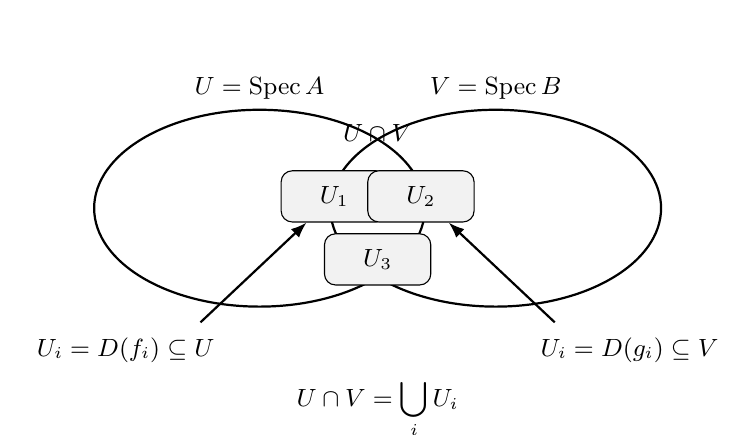
\begin{tikzpicture}[
	scale=1,
	every node/.style={font=\small},
	open/.style={draw, ellipse, minimum width=4.2cm, minimum height=2.5cm, thick},
	smallopen/.style={draw, rounded corners, fill=gray!10, minimum width=1.35cm, minimum height=0.65cm},
	arrow/.style={-{Latex[length=2mm]}, thick}
	]
	
	\node[open, label=above:{\(U=\Spec A\)}] (U) at (-1.5,0) {};
	\node[open, label=above:{\(V=\Spec B\)}] (V) at (1.5,0) {};
	
	\node at (0,0.95) {\(U\cap V\)};
	
	\node[smallopen] (Ui1) at (-0.55,0.15) {\(U_1\)};
	\node[smallopen] (Ui2) at (0.55,0.15) {\(U_2\)};
	\node[smallopen] (Ui3) at (0,-0.65) {\(U_3\)};
	
	\node at (-3.2,-1.8) {\(U_i=D(f_i)\subseteq U\)};
	\node at (3.2,-1.8) {\(U_i=D(g_i)\subseteq V\)};
	
	\draw[arrow] (-2.25,-1.45) -- (Ui1);
	\draw[arrow] (2.25,-1.45) -- (Ui2);
	
	\node at (0,-2.55) {
		\(\displaystyle U\cap V=\bigcup_i U_i\)
	};
	
\end{tikzpicture}
\]

The meaning is:

\[
\boxed{
	\text{On each }U_i,\text{ both coordinate systems are valid.}
}
\]

\subsection{Distinguished Open Dictionary}

Problem 2 is mostly about the behavior of distinguished open subsets.

\begin{center}
	\renewcommand{\arraystretch}{1.15}
	\setlength{\tabcolsep}{6pt}
	
	\begin{tabular}{c|c|>{\raggedright\arraybackslash}p{6cm}}
		\toprule
		\textbf{Geometric object} & \textbf{Algebraic object} & \textbf{Meaning} \\
		\midrule
		\(\Spec A\)
		&
		\(A\)
		&
		An affine scheme is controlled by its coordinate ring.
		\\
		\midrule
		\(D(f)\subseteq \Spec A\)
		&
		\(A_f\)
		&
		Restricting to \(D(f)\) means inverting \(f\).
		\\
		\midrule
		\(D(f)\cap D(g)\)
		&
		\(A_{fg}\)
		&
		Being in both opens means inverting both \(f\) and \(g\).
		\\
		\midrule
		\(D(f_1)\cup\cdots\cup D(f_r)=\Spec A\)
		&
		\((f_1,\dots,f_r)=A\)
		&
		The functions \(f_1,\dots,f_r\) have no common zero.
		\\
		\bottomrule
	\end{tabular}
\end{center}

The central computational rule is:
\[
\boxed{D(f)\cap D(g)=D(fg).}
\]

\subsection{Diagram: The Standard Cover of \texorpdfstring{$\PP^1_k$}{P1_k}}

The projective line has the standard affine cover
\[
\PP^1_k = U_0 \cup U_1,
\]
where
\[
U_0 = D_+(X_0) \cong \Spec k[t], \qquad t=\frac{X_1}{X_0},
\]
and
\[
U_1 = D_+(X_1) \cong \Spec k[s], \qquad s=\frac{X_0}{X_1}.
\]
On the overlap,
\[
s=\frac{1}{t}.
\]

Therefore
\[
U_0\cap U_1=D(t)\subseteq U_0
\]
and also
\[
U_0\cap U_1=D(s)\subseteq U_1.
\]

\[
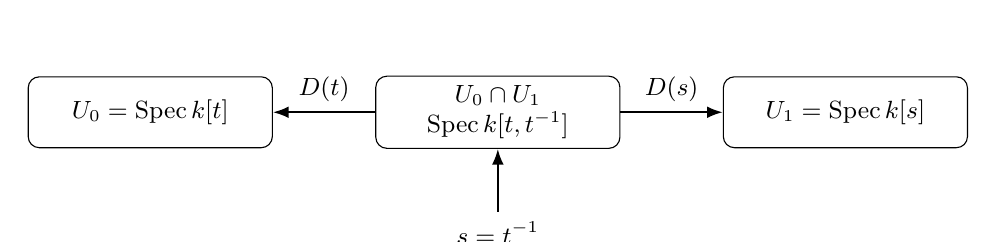
\begin{tikzpicture}[
	node distance=1.3cm,
	every node/.style={font=\small},
	box/.style={draw, rounded corners, minimum width=3.1cm, minimum height=0.9cm, align=center},
	arrow/.style={-{Latex[length=2mm]}, thick}
	]
	
	\node[box] (U0) {\(U_0=\Spec k[t]\)};
	\node[box, right=of U0] (Overlap) {\(U_0\cap U_1\)\\ \(\Spec k[t,t^{-1}]\)};
	\node[box, right=of Overlap] (U1) {\(U_1=\Spec k[s]\)};
	
	\draw[arrow] (Overlap) -- node[above] {\(D(t)\)} (U0);
	\draw[arrow] (Overlap) -- node[above] {\(D(s)\)} (U1);
	
	\node[below=0.8cm of Overlap] (trans) {\(\displaystyle s=t^{-1}\)};
	
	\draw[arrow] (trans) -- (Overlap);
	
\end{tikzpicture}
\]

Thus
\[
\boxed{
	U_0\cap U_1
	=
	D(t)\subseteq \Spec k[t]
	=
	D(s)\subseteq \Spec k[s].
}
\]

This is the standard example of gluing affine charts along a common distinguished open subset.

\subsection{Reduced, Irreducible, and Integral Schemes}

Problem 3 proves:

\[
\boxed{
	X\text{ integral}
	\iff
	X\text{ reduced and irreducible}.
}
\]

The two conditions have different meanings.

\[
\begin{array}{c|c|c}
	\toprule
	\textbf{Property} & \textbf{Algebraic meaning} & \textbf{Geometric meaning} \\
	\midrule
	Reduced
	&
	No nonzero nilpotents
	&
	No infinitesimal thickening
	\\
	\midrule
	Irreducible
	&
	Nilradical is prime on affine opens
	&
	One topological component
	\\
	\midrule
	Integral
	&
	Coordinate rings are domains
	&
	One reduced algebraic component
	\\
	\bottomrule
\end{array}
\]

\subsubsection*{Diagram: Integral as Reduced plus Irreducible}

\[
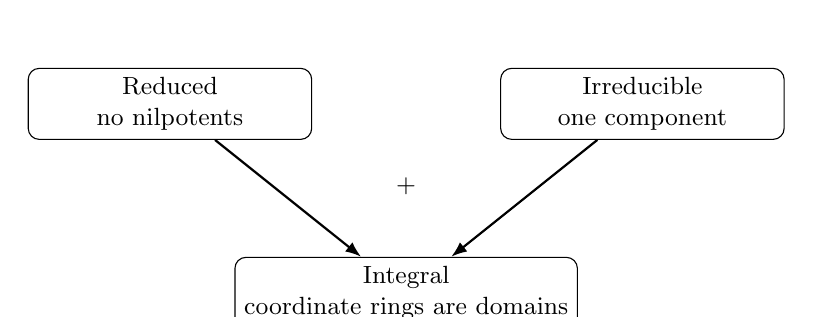
\begin{tikzpicture}[
	every node/.style={font=\small},
	box/.style={draw, rounded corners, minimum width=3.6cm, minimum height=0.9cm, align=center},
	arrow/.style={-{Latex[length=2mm]}, thick}
	]
	
	\node[box] (R) at (-3,1.3) {Reduced\\ no nilpotents};
	\node[box] (Irr) at (3,1.3) {Irreducible\\ one component};
	\node[box] (Int) at (0,-1.1) {Integral\\ coordinate rings are domains};
	
	\draw[arrow] (R) -- (Int);
	\draw[arrow] (Irr) -- (Int);
	
	\node at (0,0.25) {\(+\)};
	
\end{tikzpicture}
\]

So one should remember:

\[
\boxed{
	\text{Integral}=
	\text{no nilpotents}
	+
	\text{one component}.
}
\]

\subsection{Comparison Table: Reduced, Irreducible, Integral}

\begin{center}
	\renewcommand{\arraystretch}{1.15}
	\setlength{\tabcolsep}{6pt}
	
	\begin{tabular}{lccc}
		\toprule
		\textbf{Scheme} & \textbf{Reduced?} & \textbf{Irreducible?} & \textbf{Integral?} \\
		\midrule
		\(\Spec k[x]\) & yes & yes & yes \\
		\(\Spec k[x]/(x^2)\) & no & yes & no \\
		\(\Spec k[x,y]/(xy)\) & yes & no & no \\
		\(\Spec k[x,y]/(y^2-x^3)\) & yes & yes & yes \\
		\bottomrule
	\end{tabular}
\end{center}
This table shows why both reducedness and irreducibility are necessary.

\subsection{Table: Algebraic Meaning of Geometric Pathologies}

\[
\begin{array}{>{\raggedright\arraybackslash}p{3.4cm}
		|>{\raggedright\arraybackslash}p{3.7cm}
		|>{\raggedright\arraybackslash}p{3.5cm}
		|>{\raggedright\arraybackslash}p{3.7cm}}
	\toprule
	\textbf{Geometry} & \textbf{Algebra} & \textbf{Example} & \textbf{Effect} \\
	\midrule
	Nilpotent thickening
	&
	There exists \(a\neq 0\) with \(a^n=0\).
	&
	\(k[x]/(x^2)\)
	&
	The scheme is not reduced.
	\\
	\midrule
	Multiple components
	&
	There exist \(a,b\neq 0\) with \(ab=0\).
	&
	\(k[x,y]/(xy)\)
	&
	The scheme is reducible and not a domain.
	\\
	\midrule
	One reduced component
	&
	The zero ideal \((0)\) is prime.
	&
	\(k[x]\)
	&
	The scheme is integral.
	\\
	\midrule
	Singular but one component
	&
	The ring is a domain but not smooth.
	&
	\(k[x,y]/(y^2-x^3)\)
	&
	The scheme is integral but singular.
	\\
	\bottomrule
\end{array}
\]

This table separates three notions:

\[
\text{reduced},
\qquad
\text{irreducible},
\qquad
\text{smooth}.
\]

A singular scheme can still be integral.

\subsection{Locally Noetherian Schemes}

Problem 4 proves:

\[
\boxed{
	X\text{ locally Noetherian}
	\iff
	\text{every affine open }U=\Spec A\subseteq X\text{ has }A\text{ Noetherian}.
}
\]

This means that being locally Noetherian is independent of the chosen affine cover.

\subsubsection*{Flowchart: Proof of the Locally Noetherian Criterion}

\[
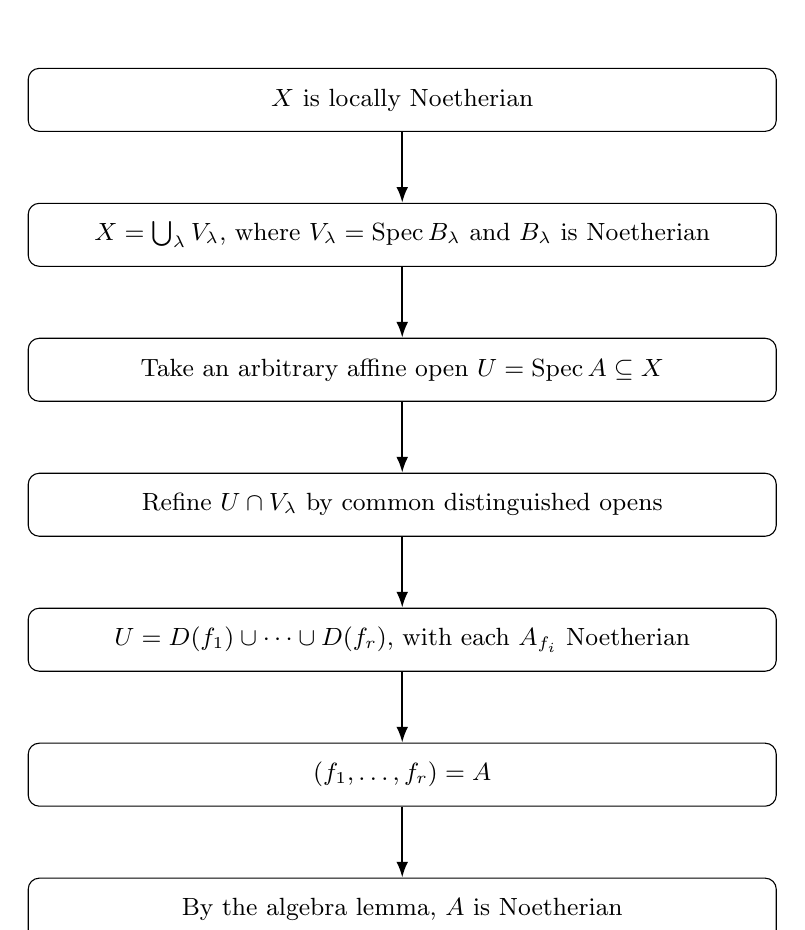
\begin{tikzpicture}[
	node distance=0.9cm,
	every node/.style={font=\small},
	box/.style={draw, rounded corners, align=center, minimum width=9.5cm, minimum height=0.8cm},
	arrow/.style={-{Latex[length=2mm]}, thick}
	]
	
	\node[box] (A) {\(X\) is locally Noetherian};
	\node[box, below=of A] (B) {\(X=\bigcup_\lambda V_\lambda\), where \(V_\lambda=\Spec B_\lambda\) and \(B_\lambda\) is Noetherian};
	\node[box, below=of B] (C) {Take an arbitrary affine open \(U=\Spec A\subseteq X\)};
	\node[box, below=of C] (D) {Refine \(U\cap V_\lambda\) by common distinguished opens};
	\node[box, below=of D] (E) {\(U=D(f_1)\cup\cdots\cup D(f_r)\), with each \(A_{f_i}\) Noetherian};
	\node[box, below=of E] (F) {\((f_1,\dots,f_r)=A\)};
	\node[box, below=of F] (G) {By the algebra lemma, \(A\) is Noetherian};
	
	\draw[arrow] (A) -- (B);
	\draw[arrow] (B) -- (C);
	\draw[arrow] (C) -- (D);
	\draw[arrow] (D) -- (E);
	\draw[arrow] (E) -- (F);
	\draw[arrow] (F) -- (G);
	
\end{tikzpicture}
\]

The proof uses three ingredients:

\[
\boxed{
	\text{affine overlap refinement}
	+
	\text{quasi-compactness}
	+
	\text{localization lemma}.
}
\]

\subsection{Locally Noetherian versus Noetherian}

\[
\begin{array}{>{\raggedright\arraybackslash}p{4.5cm}
		|c|c
		|>{\raggedright\arraybackslash}p{5.2cm}}
	\toprule
	\textbf{Scheme} & \textbf{Locally Noetherian?} & \textbf{Noetherian?} & \textbf{Reason} \\
	\midrule
	\(\Spec k[x_1,\dots,x_n]\)
	&
	yes
	&
	yes
	&
	It has one Noetherian affine chart.
	\\
	\midrule
	\(\Pj^n_k\)
	&
	yes
	&
	yes
	&
	It has a finite affine cover by copies of \(\A^n_k\).
	\\
	\midrule
	\(\displaystyle \coprod_{n\geq 1}\Spec k\)
	&
	yes
	&
	no
	&
	Each point is Noetherian, but there are infinitely many components.
	\\
	\midrule
	\(\Spec k[x_1,x_2,x_3,\dots]\)
	&
	no
	&
	no
	&
	The coordinate ring is not Noetherian.
	\\
	\bottomrule
\end{array}
\]

This table separates:

\[
\boxed{
	\text{local finite algebraic complexity}
}
\]
from
\[
\boxed{
	\text{global finite cover by such pieces}.
}
\]

\subsection{Dependency Table for Problems 2--4}

\[
\begin{array}{c|>{\raggedright\arraybackslash}p{4.8cm}|>{\raggedright\arraybackslash}p{5.6cm}}
	\toprule
	\textbf{Problem} & \textbf{Key tool} & \textbf{What it proves} \\
	\midrule
	Problem 2
	&
	Distinguished opens form a basis of affine schemes.
	&
	Affine overlaps can be refined by common distinguished opens.
	\\
	\midrule
	Problem 3
	&
	\(\Spec A\) is integral if and only if \(A\) is a domain.
	&
	A scheme is integral exactly when it is reduced and irreducible.
	\\
	\midrule
	Problem 4
	&
	Problem 2, quasi-compactness of affine schemes, and the algebra lemma on localizations.
	&
	Locally Noetherian is independent of the chosen affine cover.
	\\
	\bottomrule
\end{array}
\]

This shows that Problem 4 depends strongly on the overlap refinement from Problem 2.

\subsection{Final Summary Diagram}

\[
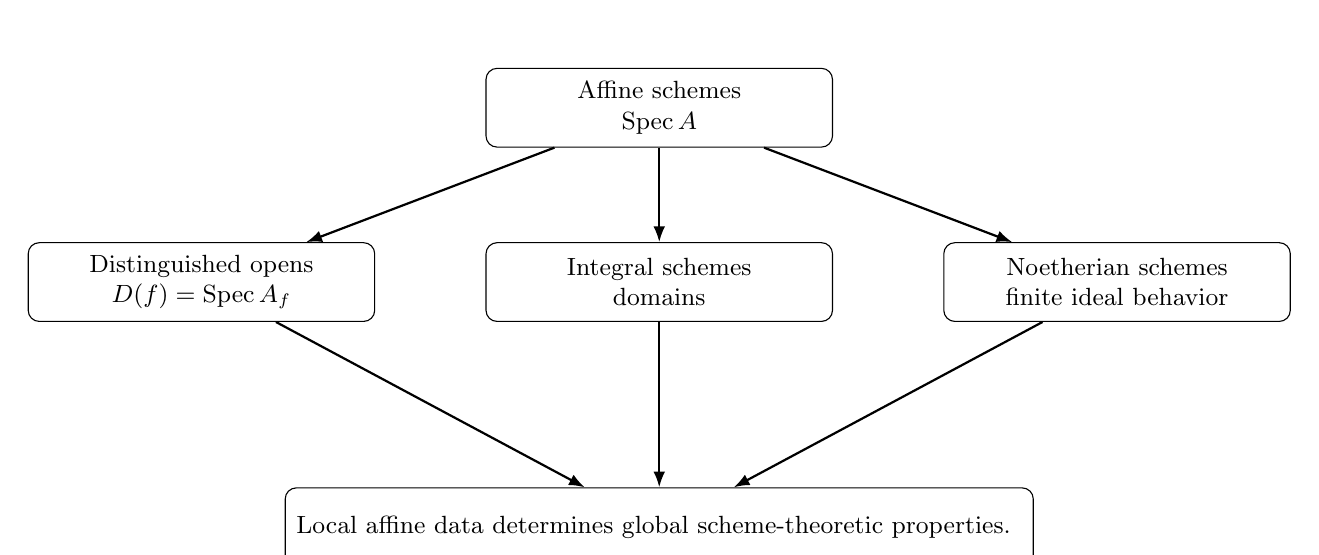
\begin{tikzpicture}[
	every node/.style={font=\small},
	box/.style={draw, rounded corners, align=center, minimum width=4.4cm, minimum height=1cm},
	arrow/.style={-{Latex[length=2mm]}, thick},
	node distance=1.2cm
	]
	
	\node[box] (Affine) {Affine schemes\\ \(\Spec A\)};
	\node[box, below left=1.2cm and 1.4cm of Affine] (Overlap) {Distinguished opens\\ \(D(f)=\Spec A_f\)};
	\node[box, below=1.2cm of Affine] (Integral) {Integral schemes\\ domains};
	\node[box, below right=1.2cm and 1.4cm of Affine] (Noeth) {Noetherian schemes\\ finite ideal behavior};
	
	\node[box, below=2.1cm of Integral, minimum width=9.5cm] (Principle) {
		Local affine data determines global scheme-theoretic properties.
	};
	
	\draw[arrow] (Affine) -- (Overlap);
	\draw[arrow] (Affine) -- (Integral);
	\draw[arrow] (Affine) -- (Noeth);
	
	\draw[arrow] (Overlap) -- (Principle);
	\draw[arrow] (Integral) -- (Principle);
	\draw[arrow] (Noeth) -- (Principle);
	
\end{tikzpicture}
\]

The main principle is:

\[
\boxed{
	\text{Schemes are controlled by affine opens, and affine opens are controlled by rings.}
}
\]

Thus, in these problems, scheme theory becomes explicit commutative algebra:

\[
\boxed{
	\text{geometry of schemes}
	\quad\longleftrightarrow\quad
	\text{commutative algebra of rings}.
}
\]

\section{Problem 5: Locally of finite type on every affine open}

\textbf{Problem.}
A morphism \(f:X\to Y\) is \emph{locally of finite type} if there exists a covering of \(Y\) by open affine subsets
\[
V_i=\Spec B_i
\]
such that, for each \(i\), \(f^{-1}(V_i)\) can be covered by open affine subsets
\[
U_{ij}=\Spec A_{ij},
\]
where each \(A_{ij}\) is a finitely generated \(B_i\)-algebra.

The morphism is \emph{of finite type} if the cover of \(f^{-1}(V_i)\) above can be taken to be finite.

Show that a morphism \(f:X\to Y\) is locally of finite type if and only if for every open affine subset
\[
V=\Spec B
\]
of \(Y\), \(f^{-1}(V)\) can be covered by open affine subsets
\[
U_j=\Spec A_j,
\]
where each \(A_j\) is a finitely generated \(B\)-algebra.

\bigskip

\textbf{Solution.}

We prove both directions.

\subsection*{First direction}

Assume that \(f:X\to Y\) is locally of finite type.

By definition, there exists an affine open covering
\[
Y=\bigcup_i V_i,
\qquad
V_i=\Spec B_i,
\]
such that, for each \(i\),
\[
f^{-1}(V_i)=\bigcup_j U_{ij},
\qquad
U_{ij}=\Spec A_{ij},
\]
and each \(A_{ij}\) is a finitely generated \(B_i\)-algebra.

Let now
\[
V=\Spec B
\]
be an arbitrary open affine subset of \(Y\). We must show that \(f^{-1}(V)\) admits a covering by affine opens whose coordinate rings are finitely generated \(B\)-algebras.

Since the \(V_i\) cover \(Y\), the open subsets
\[
V\cap V_i
\]
cover \(V\). Although \(V\cap V_i\) need not itself be affine in a general scheme, it can be covered by affine opens which are distinguished both in \(V\) and in \(V_i\). Thus, for each \(i\), we may cover \(V\cap V_i\) by open affine subsets
\[
W_{i\alpha}
\]
such that
\[
W_{i\alpha}=D(b_{i\alpha})\subseteq V=\Spec B
\]
and also
\[
W_{i\alpha}=D(c_{i\alpha})\subseteq V_i=\Spec B_i.
\]

Therefore
\[
W_{i\alpha}\cong \Spec B_{b_{i\alpha}}
\]
as an open subset of \(V\), and
\[
W_{i\alpha}\cong \Spec (B_i)_{c_{i\alpha}}
\]
as an open subset of \(V_i\).

Now consider the inverse image
\[
f^{-1}(W_{i\alpha})\subseteq f^{-1}(V_i).
\]
Since \(f^{-1}(V_i)\) is covered by the affine opens
\[
U_{ij}=\Spec A_{ij},
\]
the sets
\[
U_{ij}\cap f^{-1}(W_{i\alpha})
\]
cover \(f^{-1}(W_{i\alpha})\).

Inside \(U_{ij}=\Spec A_{ij}\), the inverse image of the distinguished open
\[
W_{i\alpha}=D(c_{i\alpha})\subseteq \Spec B_i
\]
is the distinguished open
\[
D(\varphi(c_{i\alpha}))\subseteq \Spec A_{ij},
\]
where
\[
\varphi:B_i\to A_{ij}
\]
is the ring map induced by the morphism on this affine piece.

Hence
\[
U_{ij}\cap f^{-1}(W_{i\alpha})
\cong
\Spec (A_{ij})_{\varphi(c_{i\alpha})}.
\]

Since \(A_{ij}\) is a finitely generated \(B_i\)-algebra, its localization
\[
(A_{ij})_{\varphi(c_{i\alpha})}
\]
is a finitely generated \((B_i)_{c_{i\alpha}}\)-algebra.

But
\[
(B_i)_{c_{i\alpha}}\cong B_{b_{i\alpha}},
\]
because both are coordinate rings of the same affine open subset \(W_{i\alpha}\).

Therefore
\[
(A_{ij})_{\varphi(c_{i\alpha})}
\]
is a finitely generated \(B_{b_{i\alpha}}\)-algebra.

Finally,
\[
B_{b_{i\alpha}}
\]
is a finitely generated \(B\)-algebra, because
\[
B_{b_{i\alpha}}\cong B[t]/(b_{i\alpha}t-1).
\]
Therefore any finitely generated \(B_{b_{i\alpha}}\)-algebra is also a finitely generated \(B\)-algebra.

So each affine open
\[
U_{ij}\cap f^{-1}(W_{i\alpha})
\]
has coordinate ring finitely generated over \(B\).

Since the opens \(W_{i\alpha}\) cover \(V\), their inverse images cover \(f^{-1}(V)\). Therefore the affine opens
\[
U_{ij}\cap f^{-1}(W_{i\alpha})
\]
cover \(f^{-1}(V)\), and each has coordinate ring finitely generated over \(B\).

Thus, for every affine open
\[
V=\Spec B\subseteq Y,
\]
the inverse image \(f^{-1}(V)\) can be covered by affine opens
\[
\Spec A_j
\]
with each \(A_j\) a finitely generated \(B\)-algebra.

\subsection*{Second direction}

Conversely, assume that for every affine open subset
\[
V=\Spec B\subseteq Y,
\]
the inverse image \(f^{-1}(V)\) can be covered by affine opens
\[
U_j=\Spec A_j,
\]
where each \(A_j\) is a finitely generated \(B\)-algebra.

Choose any affine open covering
\[
Y=\bigcup_i V_i,
\qquad
V_i=\Spec B_i.
\]
By assumption, for each \(i\), the inverse image
\[
f^{-1}(V_i)
\]
can be covered by affine opens
\[
U_{ij}=\Spec A_{ij},
\]
where each \(A_{ij}\) is a finitely generated \(B_i\)-algebra.

But this is exactly the definition of \(f\) being locally of finite type.

Therefore \(f\) is locally of finite type.

\subsection*{Conclusion}

We have proved that \(f:X\to Y\) is locally of finite type if and only if for every affine open subset
\[
V=\Spec B\subseteq Y,
\]
the inverse image \(f^{-1}(V)\) can be covered by affine open subsets
\[
U_j=\Spec A_j
\]
such that each \(A_j\) is a finitely generated \(B\)-algebra.

\section{Problem 6: Examples violating the properties}

\textbf{Problem.}
For each of the properties defined above of schemes or morphisms, give an example of a scheme or morphism which violates that property. Give an example of a morphism which is locally of finite type but not of finite type.

\bigskip

\textbf{Solution.}

We list standard examples.

\subsection*{A scheme which is not reduced}

Let
\[
X=\Spec k[\varepsilon]/(\varepsilon^2).
\]
The ring
\[
k[\varepsilon]/(\varepsilon^2)
\]
has a nonzero nilpotent element, namely \(\varepsilon\), because
\[
\varepsilon\neq 0,
\qquad
\varepsilon^2=0.
\]
Therefore the ring is not reduced.

Hence
\[
\Spec k[\varepsilon]/(\varepsilon^2)
\]
is a scheme which is not reduced.

\subsection*{A scheme which is not irreducible}

Let
\[
X=\Spec k[x,y]/(xy).
\]
Geometrically, this is the union of the two coordinate axes in the affine plane.

Indeed, in \(\mathbb A_k^2=\Spec k[x,y]\), the equation
\[
xy=0
\]
means
\[
x=0
\qquad\text{or}\qquad
y=0.
\]
Thus
\[
\Spec k[x,y]/(xy)
\]
is the union of the closed subsets
\[
V(x)
\qquad\text{and}\qquad
V(y).
\]
Both are proper closed subsets. Therefore \(X\) is reducible.

Hence
\[
X=\Spec k[x,y]/(xy)
\]
is not irreducible.

\subsection*{A scheme which is not integral}

A scheme is integral if it is both reduced and irreducible.

Thus either a non-reduced scheme or a reducible scheme gives an example of a non-integral scheme.

For example,
\[
X=\Spec k[x,y]/(xy)
\]
is reduced but reducible. Therefore it is not integral.

Another example is
\[
X=\Spec k[\varepsilon]/(\varepsilon^2),
\]
which is not reduced. Hence it is not integral.

\subsection*{A morphism which is not locally of finite type}

Consider the morphism
\[
f:\Spec k[x_1,x_2,x_3,\dots]\longrightarrow \Spec k.
\]
This morphism corresponds to the inclusion
\[
k\longrightarrow k[x_1,x_2,x_3,\dots].
\]

The ring
\[
k[x_1,x_2,x_3,\dots]
\]
is not a finitely generated \(k\)-algebra, because it has infinitely many algebraically independent variables.

Since the target is affine,
\[
\Spec k,
\]
the definition of locally finite type would require the source to be covered by affine opens whose coordinate rings are finitely generated \(k\)-algebras.

But the whole source is
\[
\Spec k[x_1,x_2,x_3,\dots],
\]
and the algebra contains infinitely many independent variables. This is the standard example of a morphism which is not locally of finite type.

Therefore
\[
\Spec k[x_1,x_2,x_3,\dots]\longrightarrow \Spec k
\]
is not locally of finite type.

\subsection*{A morphism which is locally of finite type but not of finite type}

Let
\[
X=\coprod_{n\geq 1}\mathbb A_k^1
\]
be a countably infinite disjoint union of affine lines over \(k\). Consider the natural morphism
\[
f:X\longrightarrow \Spec k.
\]

Each component is
\[
\mathbb A_k^1=\Spec k[t],
\]
and \(k[t]\) is a finitely generated \(k\)-algebra. Therefore each component is of finite type over \(\Spec k\).

The inverse image of the only affine open of \(\Spec k\) is
\[
f^{-1}(\Spec k)=X.
\]
This is covered by the affine opens
\[
\mathbb A_k^1,\mathbb A_k^1,\mathbb A_k^1,\dots
\]
one for each component. On each such open, the coordinate ring is \(k[t]\), which is finitely generated over \(k\).

Therefore \(f\) is locally of finite type.

However, \(X\) cannot be covered by finitely many of these connected components. Indeed, a finite union of components would miss all the remaining components. Hence \(X\) is not quasi-compact.

Since a morphism of finite type is, in particular, quasi-compact, this morphism cannot be of finite type.

Therefore
\[
\coprod_{n\geq 1}\mathbb A_k^1
\longrightarrow
\Spec k
\]
is locally of finite type but not of finite type.

\subsection*{A scheme which is not a variety}

In the language of the remark, a variety over an algebraically closed field \(k\) is an integral scheme of finite type over \(\Spec k\).

Thus a scheme can fail to be a variety in several ways.

For example,
\[
\Spec k[\varepsilon]/(\varepsilon^2)
\]
is not a variety because it is not reduced.

Also,
\[
\Spec k[x,y]/(xy)
\]
is not a variety because it is reducible, hence not integral.

Finally,
\[
\Spec k[x_1,x_2,x_3,\dots]
\]
is not a variety because it is not of finite type over \(k\).

\subsection*{Summary of examples}

\[
\begin{array}{c|c}
	\textbf{Property violated} & \textbf{Example} \\
	\hline
	\text{Reduced} &
	\Spec k[\varepsilon]/(\varepsilon^2)
	\\[4pt]
	\text{Irreducible} &
	\Spec k[x,y]/(xy)
	\\[4pt]
	\text{Integral} &
	\Spec k[x,y]/(xy)
	\\[4pt]
	\text{Locally of finite type} &
	\Spec k[x_1,x_2,x_3,\dots]\to \Spec k
	\\[4pt]
	\text{Finite type} &
	\displaystyle \coprod_{n\geq 1}\mathbb A_k^1\to \Spec k
	\\[8pt]
	\text{Variety over }k &
	\Spec k[\varepsilon]/(\varepsilon^2)
\end{array}
\]

\section{Problem 7: Generic point and function field of an integral scheme}

\textbf{Problem.}
Let \(X\) be an integral scheme. Show that there is a unique point \(\eta\) such that the closure of \(\{\eta\}\) is \(X\); this is called the \emph{generic point} of \(X\). Show that the stalk of \(\OO_X\) at \(\eta\) is a field, called the \emph{function field} of \(X\), denoted by \(K(X)\). Show that if
\[
U=\Spec A
\]
is any open affine subset of \(X\), then \(K(X)\) is the field of fractions of \(A\).

\bigskip

\textbf{Solution.}

Since \(X\) is integral, it is nonempty, reduced, and irreducible. In particular, every nonempty open subset of \(X\) is dense in \(X\), and every nonempty affine open subset has coordinate ring an integral domain.

\subsection*{Existence of the generic point}

Choose a nonempty affine open subset
\[
U=\Spec A\subseteq X.
\]
Since \(X\) is integral, the open subscheme \(U\) is also integral. Hence its coordinate ring \(A\) is an integral domain.

Because \(A\) is a domain, the zero ideal
\[
(0)\subseteq A
\]
is a prime ideal. Therefore it determines a point
\[
\eta=(0)\in \Spec A.
\]

In the affine scheme \(\Spec A\), the closure of the point corresponding to a prime ideal \(\mathfrak p\) is
\[
\overline{\{\mathfrak p\}}=V(\mathfrak p).
\]
Thus
\[
\overline{\{(0)\}}=V((0))=\Spec A.
\]
So \((0)\) is the generic point of \(U\).

We now show that this same point is generic for all of \(X\).

Let \(W\subseteq X\) be a nonempty open subset. Since \(X\) is irreducible, any two nonempty open subsets of \(X\) intersect. Therefore
\[
W\cap U\neq \varnothing.
\]
But \(W\cap U\) is a nonempty open subset of \(U=\Spec A\). Since \((0)\) is the generic point of \(U\), it lies in every nonempty open subset of \(U\). Hence
\[
\eta\in W\cap U\subseteq W.
\]
Therefore \(\eta\) lies in every nonempty open subset of \(X\).

Equivalently, the closure of \(\{\eta\}\) is all of \(X\):
\[
\overline{\{\eta\}}=X.
\]
Thus \(X\) has a generic point.

\subsection*{Uniqueness of the generic point}

Suppose that \(\eta\) and \(\eta'\) are two points of \(X\) satisfying
\[
\overline{\{\eta\}}=X
\qquad\text{and}\qquad
\overline{\{\eta'\}}=X.
\]
Then both \(\eta\) and \(\eta'\) lie in every nonempty open subset of \(X\).

Schemes are \(T_0\)-spaces. This means that if two points are distinct, then there exists an open subset containing one of them but not the other.

Assume, for contradiction, that
\[
\eta\neq \eta'.
\]
Then there is an open subset \(W\subseteq X\) containing one of the two points but not the other. Since \(W\) contains one of the points, it is nonempty. But every nonempty open subset of \(X\) must contain both \(\eta\) and \(\eta'\), because both have dense closure equal to \(X\). This is a contradiction.

Therefore
\[
\eta=\eta'.
\]
So the generic point of \(X\) is unique.

\subsection*{The stalk at the generic point is a field}

Let
\[
U=\Spec A
\]
be an affine open neighborhood of \(\eta\). Since \(X\) is integral, \(A\) is an integral domain.

Inside \(U=\Spec A\), the point \(\eta\) corresponds to the prime ideal
\[
(0)\subseteq A.
\]
Therefore the stalk of the structure sheaf at \(\eta\) is
\[
\OO_{X,\eta}
\cong
\OO_{U,\eta}
\cong
A_{(0)}.
\]

But localizing an integral domain \(A\) at the zero prime ideal means inverting all nonzero elements of \(A\). Hence
\[
A_{(0)}=\Frac(A).
\]
Therefore
\[
\OO_{X,\eta}
\]
is a field.

This field is called the function field of \(X\), and is denoted
\[
K(X):=\OO_{X,\eta}.
\]

\subsection*{The function field on any affine open}

Let
\[
U=\Spec A
\]
be any nonempty affine open subset of \(X\).

Since \(\eta\) is the generic point of \(X\), it lies in every nonempty open subset of \(X\). In particular,
\[
\eta\in U.
\]
Since \(X\) is integral, the affine scheme \(U\) is integral, and therefore \(A\) is an integral domain.

In \(\Spec A\), the generic point corresponds to the zero ideal
\[
(0)\subseteq A.
\]
Thus
\[
K(X)
=
\OO_{X,\eta}
\cong
\OO_{U,\eta}
\cong
A_{(0)}
=
\Frac(A).
\]

Therefore, for every nonempty affine open subset
\[
U=\Spec A\subseteq X,
\]
we have
\[
K(X)\cong \Frac(A).
\]

\subsection*{Conclusion}

For an integral scheme \(X\), there exists a unique point
\[
\eta\in X
\]
such that
\[
\overline{\{\eta\}}=X.
\]
This point is called the generic point of \(X\).

The stalk at this point,
\[
K(X):=\OO_{X,\eta},
\]
is a field, called the function field of \(X\).

Moreover, for every nonempty affine open subset
\[
U=\Spec A\subseteq X,
\]
there is a canonical identification
\[
K(X)\cong \Frac(A).
\]

\section{Theory for Problems 5--7}

This section collects the main theory behind Problems 5--7. The common theme is that many important properties of schemes and morphisms are \emph{local on affine opens}. In particular, finite generation of coordinate rings controls morphisms of finite type, while integrality controls the existence of a generic point and the construction of the function field.

\subsection{Locally finite type and finite type morphisms}

Let
\[
f:X\to Y
\]
be a morphism of schemes.

\textbf{Definition.}
The morphism \(f\) is called \emph{locally of finite type} if there exists an affine open covering
\[
Y=\bigcup_i V_i,
\qquad
V_i=\Spec B_i,
\]
such that for each \(i\), the inverse image \(f^{-1}(V_i)\) can be covered by affine open subsets
\[
U_{ij}=\Spec A_{ij},
\]
where each \(A_{ij}\) is a finitely generated \(B_i\)-algebra.

Equivalently, locally on the target and locally on the source, the morphism looks like a ring map
\[
B_i\to A_{ij}
\]
where \(A_{ij}\) is generated over \(B_i\) by finitely many elements.

\medskip

\textbf{Definition.}
The morphism \(f\) is called \emph{of finite type} if, in the definition above, the covering of each \(f^{-1}(V_i)\) by affine open subsets
\[
U_{ij}=\Spec A_{ij}
\]
can be chosen to be finite.

Thus:

\[
\text{finite type}
\quad =
\quad
\text{locally finite type}
\quad +
\quad
\text{finite covering condition}.
\]

More conceptually, finite type morphisms are the geometric analogue of finitely generated algebras.

\subsection{Affine algebraic meaning}

The basic affine model is this.

Let
\[
f:\Spec A\to \Spec B
\]
be a morphism of affine schemes. Such a morphism corresponds contravariantly to a ring homomorphism
\[
B\to A.
\]

Then \(f\) is of finite type precisely when \(A\) is a finitely generated \(B\)-algebra.

This means that there exist elements
\[
a_1,\dots,a_n\in A
\]
such that
\[
A=B[a_1,\dots,a_n].
\]
Equivalently, there is a surjective \(B\)-algebra homomorphism
\[
B[x_1,\dots,x_n]\twoheadrightarrow A.
\]

So the affine schemes of finite type over \(\Spec B\) are exactly those built from finitely many algebraic coordinates over \(B\).

\subsection{Why the condition is local}

The property of being locally of finite type is local on the target.

This means that it is enough to check the property on one affine open covering of \(Y\), and then it automatically holds on every affine open subset of \(Y\).

The key reason is that affine opens can be refined by smaller affine opens. More precisely, if
\[
V=\Spec B
\]
is an affine open subset of \(Y\), and \(V_i=\Spec B_i\) is another affine open subset, then the intersection
\[
V\cap V_i
\]
can be covered by smaller affine open subsets. Around any point of \(V\cap V_i\), one can choose an affine open subset contained in both \(V\) and \(V_i\).

In practice, one refines the intersection by distinguished opens. For example, inside
\[
V=\Spec B,
\]
a distinguished open has the form
\[
D(b)=\Spec B_b.
\]

The coordinate ring \(B_b\) is a finitely generated \(B\)-algebra because
\[
B_b\cong B[t]/(bt-1).
\]

This simple fact is crucial: localizing at one element does not destroy finite generation over the original base ring.

\subsection{Localization preserves finite generation}

A basic algebraic fact used repeatedly is the following.

\medskip

\textbf{Lemma.}
Let \(A\) be a finitely generated \(B\)-algebra, and let \(S\subseteq B\) be a multiplicative subset. Then
\[
S^{-1}A
\]
is a finitely generated \(S^{-1}B\)-algebra.

\medskip

\textbf{Reason.}
If
\[
A=B[a_1,\dots,a_n],
\]
then after localization,
\[
S^{-1}A=(S^{-1}B)[a_1/1,\dots,a_n/1].
\]
Thus the same generators still generate after localization.

In particular, if \(b\in B\), then
\[
A_b
\]
is a finitely generated \(B_b\)-algebra.

Also, since
\[
B_b\cong B[t]/(bt-1),
\]
the ring \(B_b\) is a finitely generated \(B\)-algebra. Hence a finitely generated \(B_b\)-algebra is also finitely generated over \(B\).

This explains the mechanism behind Problem 5.

\subsection{Geometric meaning of finite type}

A morphism
\[
f:X\to Y
\]
of finite type should be thought of as a family of geometric objects over \(Y\) which can be described using finitely many algebraic coordinates and finitely many affine charts.

For example, over a field \(k\), a scheme of finite type over \(\Spec k\) is locally described by rings of the form
\[
k[x_1,\dots,x_n]/I.
\]
Thus finite type schemes over \(k\) are the schemes that behave like algebraic sets cut out in finite-dimensional affine space.

By contrast,
\[
\Spec k[x_1,x_2,x_3,\dots]
\]
is not of finite type over \(k\), because its coordinate ring needs infinitely many independent variables.

\subsection{Locally finite type versus finite type}

The difference between \emph{locally of finite type} and \emph{of finite type} is a finiteness condition on the number of affine pieces needed.

A morphism may be locally finite type because every small affine piece is finitely generated over the base, but it may fail to be finite type because infinitely many such pieces are needed.

The standard example is
\[
X=\coprod_{n\geq 1}\mathbb A_k^1
\]
with the natural morphism
\[
X\to \Spec k.
\]

Each component
\[
\mathbb A_k^1=\Spec k[t]
\]
is of finite type over \(k\), so the morphism is locally of finite type.

However, the source is an infinite disjoint union, so it is not quasi-compact. Therefore it cannot be of finite type.

Thus:

\[
\coprod_{n\geq 1}\mathbb A_k^1\to \Spec k
\]
is locally of finite type but not of finite type.

\subsection{Reduced, irreducible, and integral schemes}

The examples in Problem 6 depend on the basic properties of schemes.

\medskip

\textbf{Reduced schemes.}
A scheme \(X\) is reduced if, for every open subset \(U\subseteq X\), the ring
\[
\OO_X(U)
\]
has no nonzero nilpotent elements.

Affine-locally, this means that if
\[
X=\Spec A,
\]
then \(X\) is reduced precisely when \(A\) is a reduced ring.

For example,
\[
\Spec k[\varepsilon]/(\varepsilon^2)
\]
is not reduced because
\[
\varepsilon\neq 0,
\qquad
\varepsilon^2=0.
\]

\medskip

\textbf{Irreducible schemes.}
A topological space \(X\) is irreducible if it cannot be written as the union of two proper closed subsets.

Equivalently, every two nonempty open subsets of \(X\) intersect.

For affine schemes,
\[
\Spec A
\]
is irreducible if and only if the nilradical of \(A\) is a prime ideal. In particular, if \(A\) is a domain, then \(\Spec A\) is irreducible.

For example,
\[
\Spec k[x,y]/(xy)
\]
is reducible because it is the union of the two coordinate axes:
\[
V(xy)=V(x)\cup V(y).
\]

\medskip

\textbf{Integral schemes.}
A scheme \(X\) is integral if it is both reduced and irreducible.

Affine-locally, an affine scheme
\[
\Spec A
\]
is integral if and only if \(A\) is an integral domain.

So:
\[
\Spec A \text{ integral}
\quad\Longleftrightarrow\quad
A \text{ is a domain}.
\]

\subsection{Varieties in this language}

In the language of these exercises, a variety over an algebraically closed field \(k\) is an integral scheme of finite type over
\[
\Spec k.
\]

Thus a \(k\)-variety must satisfy two kinds of conditions:

\[
\begin{array}{c|c}
	\textbf{Condition} & \textbf{Meaning} \\
	\hline
	\text{Integral} & \text{Geometrically one reduced irreducible piece} \\
	\text{Finite type over }k & \text{Described by finitely many algebraic coordinates over }k
\end{array}
\]

Therefore the following are not varieties:

\[
\Spec k[\varepsilon]/(\varepsilon^2),
\]
because it is not reduced;

\[
\Spec k[x,y]/(xy),
\]
because it is reducible;

and

\[
\Spec k[x_1,x_2,x_3,\dots],
\]
because it is not of finite type over \(k\).

\subsection{Generic points}

Let \(X\) be an integral scheme.

Because \(X\) is irreducible, it has a unique dense irreducible component: namely \(X\) itself.

A point
\[
\eta\in X
\]
is called a \emph{generic point} of \(X\) if
\[
\overline{\{\eta\}}=X.
\]

For an affine integral scheme
\[
X=\Spec A,
\]
where \(A\) is a domain, the generic point is the point corresponding to the zero ideal:
\[
\eta=(0).
\]

Indeed, since \(A\) is a domain, \((0)\) is a prime ideal. Its closure is
\[
\overline{\{(0)\}}=V((0))=\Spec A.
\]

Thus \((0)\) is dense in \(\Spec A\).

\subsection{Generic point of an integral scheme}

For a general integral scheme \(X\), choose a nonempty affine open subset
\[
U=\Spec A\subseteq X.
\]
Since \(X\) is integral, the ring \(A\) is a domain. Therefore \(U\) has generic point
\[
(0)\in \Spec A.
\]

This point is also the generic point of all of \(X\).

The reason is that \(X\) is irreducible. Hence every nonempty open subset of \(X\) intersects \(U\). Since \((0)\) lies in every nonempty open subset of \(U\), it lies in every nonempty open subset of \(X\).

Therefore
\[
\overline{\{\eta\}}=X.
\]

The generic point is unique because schemes are \(T_0\)-spaces: two distinct points can be topologically distinguished by an open set. If two points both had closure equal to \(X\), then both would lie in every nonempty open subset, which would contradict the \(T_0\) property unless the two points were equal.

\subsection{The stalk at the generic point}

Let \(X\) be an integral scheme with generic point \(\eta\).

The stalk
\[
\OO_{X,\eta}
\]
is the local ring of \(X\) at the generic point.

If
\[
U=\Spec A
\]
is an affine open neighborhood of \(\eta\), then \(\eta\) corresponds to the prime ideal
\[
(0)\subseteq A.
\]
Therefore
\[
\OO_{X,\eta}\cong A_{(0)}.
\]

Since \(A\) is a domain, localizing at \((0)\) means inverting every nonzero element of \(A\). Hence
\[
A_{(0)}=\Frac(A).
\]

Therefore
\[
\OO_{X,\eta}
\]
is a field.

This field is called the \emph{function field} of \(X\), and is denoted
\[
K(X).
\]

Thus
\[
K(X):=\OO_{X,\eta}.
\]

\subsection{Function field on affine opens}

If
\[
U=\Spec A
\]
is any nonempty affine open subset of an integral scheme \(X\), then \(\eta\in U\), because the generic point lies in every nonempty open subset.

Inside \(U=\Spec A\), the point \(\eta\) corresponds to the prime ideal
\[
(0)\subseteq A.
\]

Hence
\[
K(X)=\OO_{X,\eta}\cong A_{(0)}=\Frac(A).
\]

Therefore, for every nonempty affine open subset
\[
U=\Spec A\subseteq X,
\]
we have
\[
K(X)\cong \Frac(A).
\]

This is why the function field of an integral scheme may be computed from any affine chart.

\subsection{Geometric meaning of the function field}

If \(X\) is an integral variety over a field \(k\), then \(K(X)\) is the field of rational functions on \(X\).

For example, if
\[
X=\mathbb A_k^n=\Spec k[x_1,\dots,x_n],
\]
then
\[
K(X)=\Frac(k[x_1,\dots,x_n])=k(x_1,\dots,x_n).
\]

If
\[
X=\Spec k[x,y]/(y^2-x^3-x)
\]
is an integral affine curve, then its function field is
\[
K(X)=\Frac\bigl(k[x,y]/(y^2-x^3-x)\bigr).
\]

Elements of \(K(X)\) are not necessarily regular everywhere on \(X\). They are rational functions, meaning that they are regular on some nonempty open subset of \(X\).

\subsection{Conceptual summary}

The three problems are connected as follows:

\[
\begin{array}{c|c|c}
	\textbf{Topic} & \textbf{Algebraic condition} & \textbf{Geometric meaning} \\
	\hline
	\text{Locally finite type} &
	\text{locally finitely generated algebras} &
	\text{finite-dimensional algebraic behavior locally}
	\\[4pt]
	\text{Finite type} &
	\text{finite affine cover by finitely generated algebras} &
	\text{globally finite algebraic family}
	\\[4pt]
	\text{Reduced} &
	\text{no nilpotents} &
	\text{no infinitesimal thickening}
	\\[4pt]
	\text{Irreducible} &
	\text{one topological component} &
	\text{one algebraic piece}
	\\[4pt]
	\text{Integral} &
	\text{domain on affine charts} &
	\text{reduced and irreducible}
	\\[4pt]
	\text{Generic point} &
	(0)\in \Spec A \text{ for a domain } A &
	\text{point whose closure is all of }X
	\\[4pt]
	\text{Function field} &
	\Frac(A) &
	\text{rational functions on }X
\end{array}
\]

\subsection{Main takeaways}

\[
\boxed{
	\text{Locally finite type is checked on affine opens and survives refinement.}
}
\]

\[
\boxed{
	\text{Finite type adds a global finiteness condition to local finite generation.}
}
\]

\[
\boxed{
	\text{Integral schemes have a unique generic point.}
}
\]

\[
\boxed{
	K(X)=\OO_{X,\eta}\cong \Frac(A)
	\text{ for every nonempty affine open } U=\Spec A\subseteq X.
}
\]
\section{Examples for Problems 5--7}

This section gives concrete examples illustrating the notions from Problems 5--7: locally finite type morphisms, finite type morphisms, reduced schemes, irreducible schemes, integral schemes, varieties, generic points, and function fields.

\subsection{Example 1: An affine morphism of finite type}

Let \(k\) be a field, and consider
\[
X=\operatorname{Spec} k[x,y]/(y^2-x^3-x)
\]
with the natural morphism
\[
f:X\to \operatorname{Spec} k.
\]

The coordinate ring of \(X\) is
\[
A=k[x,y]/(y^2-x^3-x).
\]

This is a finitely generated \(k\)-algebra, because it is generated by the images of \(x\) and \(y\). Indeed,
\[
A=k[\overline{x},\overline{y}].
\]

Equivalently, there is a surjective \(k\)-algebra homomorphism
\[
k[x,y]\twoheadrightarrow k[x,y]/(y^2-x^3-x).
\]

Therefore the morphism
\[
\operatorname{Spec} k[x,y]/(y^2-x^3-x)
\to
\operatorname{Spec} k
\]
is of finite type.

Geometrically, this is an affine algebraic curve over \(k\).

\subsection{Example 2: A morphism locally of finite type}

Let
\[
X=\mathbb A_k^2=\operatorname{Spec} k[x,y],
\]
and consider the natural morphism
\[
f:\mathbb A_k^2\to \operatorname{Spec} k.
\]

Since
\[
k[x,y]
\]
is a finitely generated \(k\)-algebra, the morphism is of finite type. Hence it is also locally of finite type.

Now take a distinguished open subset
\[
D(x)\subseteq \mathbb A_k^2.
\]
Its coordinate ring is
\[
k[x,y]_x.
\]

This is still finitely generated over \(k\), because
\[
k[x,y]_x\cong k[x,y,t]/(xt-1).
\]

Thus localization preserves the finite type nature of the morphism.

This example illustrates the idea from Problem 5: when we restrict to smaller affine opens, we still get finitely generated algebras.

\subsection{Example 3: Checking locally finite type on another affine open}

Let
\[
Y=\operatorname{Spec} k[s],
\]
and let
\[
X=\operatorname{Spec} k[s,t].
\]

Consider the morphism
\[
f:X\to Y
\]
induced by the inclusion
\[
k[s]\hookrightarrow k[s,t].
\]

This morphism is of finite type because
\[
k[s,t]=k[s][t],
\]
so \(k[s,t]\) is generated over \(k[s]\) by one element, namely \(t\).

Now take the distinguished open subset
\[
V=D(s)\subseteq Y.
\]
Then
\[
V=\operatorname{Spec} k[s]_s.
\]

The inverse image of \(V\) is
\[
f^{-1}(D(s))=D(s)\subseteq X.
\]
Its coordinate ring is
\[
k[s,t]_s.
\]

But
\[
k[s,t]_s\cong k[s]_s[t].
\]
So \(k[s,t]_s\) is a finitely generated \(k[s]_s\)-algebra.

Therefore the morphism remains locally of finite type after passing to the affine open subset \(D(s)\).

This is exactly the behavior described in Problem 5.

\subsection{Example 4: A morphism not locally of finite type}

Consider
\[
X=\operatorname{Spec} k[x_1,x_2,x_3,\dots]
\]
and the natural morphism
\[
f:X\to \operatorname{Spec} k.
\]

The coordinate ring
\[
k[x_1,x_2,x_3,\dots]
\]
is the polynomial ring in infinitely many variables.

This ring is not finitely generated as a \(k\)-algebra. Indeed, if it were generated by finitely many elements, then only finitely many variables could appear in those generators. But then variables outside that finite list could not be produced.

Therefore
\[
k[x_1,x_2,x_3,\dots]
\]
is not a finitely generated \(k\)-algebra.

Hence the morphism
\[
\operatorname{Spec} k[x_1,x_2,x_3,\dots]
\to
\operatorname{Spec} k
\]
is not locally of finite type.

This example shows that infinite-dimensional affine space is not of finite type over \(k\).

\subsection{Example 5: Locally of finite type but not finite type}

Let
\[
X=\coprod_{n\geq 1}\mathbb A_k^1
\]
be the infinite disjoint union of copies of the affine line over \(k\). Consider the natural morphism
\[
f:X\to \operatorname{Spec} k.
\]

Each component is
\[
\mathbb A_k^1=\operatorname{Spec} k[t],
\]
and \(k[t]\) is a finitely generated \(k\)-algebra.

Therefore every point of \(X\) has an affine open neighborhood mapping to \(\operatorname{Spec} k\) by a finite type morphism. Hence
\[
f:X\to \operatorname{Spec} k
\]
is locally of finite type.

However, \(X\) is an infinite disjoint union of nonempty open subsets. It is not quasi-compact, because no finite collection of components covers all of \(X\).

A finite type morphism is quasi-compact. Therefore
\[
f:X\to \operatorname{Spec} k
\]
is not of finite type.

Thus this is the standard example of a morphism which is locally of finite type but not finite type.

\subsection{Example 6: A non-reduced scheme}

Let
\[
X=\operatorname{Spec} k[\varepsilon]/(\varepsilon^2).
\]

In the ring
\[
k[\varepsilon]/(\varepsilon^2),
\]
the element \(\varepsilon\) satisfies
\[
\varepsilon^2=0,
\]
but
\[
\varepsilon\neq 0.
\]

Thus \(\varepsilon\) is a nonzero nilpotent element.

Therefore
\[
k[\varepsilon]/(\varepsilon^2)
\]
is not reduced, and so
\[
X=\operatorname{Spec} k[\varepsilon]/(\varepsilon^2)
\]
is not a reduced scheme.

Geometrically, this scheme is an infinitesimal thickening of a point. It has the same underlying topological space as \(\operatorname{Spec} k\), but it has extra nilpotent structure.

\subsection{Example 7: A reducible scheme}

Let
\[
X=\operatorname{Spec} k[x,y]/(xy).
\]

The equation
\[
xy=0
\]
means that either
\[
x=0
\]
or
\[
y=0.
\]

Thus \(X\) is the union of the two coordinate axes in the affine plane:
\[
X=V(x)\cup V(y).
\]

Both \(V(x)\) and \(V(y)\) are proper closed subsets of \(X\). Hence \(X\) is reducible.

Therefore
\[
\operatorname{Spec} k[x,y]/(xy)
\]
is not irreducible.

This example is reduced if \(k\) is a field, because the ideal \((xy)\) is radical in \(k[x,y]\). However, it is not integral because it is reducible.

\subsection{Example 8: A scheme that is irreducible but not reduced}

Let
\[
X=\operatorname{Spec} k[x]/(x^2).
\]

The ring
\[
k[x]/(x^2)
\]
has a nilpotent element, namely the image of \(x\), because
\[
x^2=0.
\]

So \(X\) is not reduced.

However, the underlying topological space has only one prime ideal, namely
\[
(x)/(x^2).
\]
Therefore \(X\) is irreducible as a topological space.

Thus
\[
\operatorname{Spec} k[x]/(x^2)
\]
is irreducible but not reduced.

Consequently, it is not integral.

\subsection{Example 9: A reduced scheme that is not integral}

Let
\[
X=\operatorname{Spec} k[x,y]/(xy).
\]

As above, this scheme is the union of two coordinate axes:
\[
V(xy)=V(x)\cup V(y).
\]

The ring
\[
k[x,y]/(xy)
\]
is reduced, because \((xy)\) is a radical ideal in \(k[x,y]\). But it is not a domain, since
\[
\overline{x}\cdot \overline{y}=0
\]
while
\[
\overline{x}\neq 0,
\qquad
\overline{y}\neq 0.
\]

Therefore the scheme is reduced but not integral.

This example shows that reducedness alone is not enough for integrality. We also need irreducibility.

\subsection{Example 10: A variety over an algebraically closed field}

Let \(k\) be algebraically closed, and consider
\[
X=\operatorname{Spec} k[x,y]/(y-x^2).
\]

The ring
\[
k[x,y]/(y-x^2)
\]
is isomorphic to
\[
k[x],
\]
because the relation \(y=x^2\) allows us to eliminate \(y\).

Indeed,
\[
k[x,y]/(y-x^2)\cong k[x].
\]

Since \(k[x]\) is a domain, \(X\) is integral.

Since \(k[x]\) is finitely generated over \(k\), the morphism
\[
X\to \operatorname{Spec} k
\]
is of finite type.

Therefore \(X\) is a variety over \(k\).

Geometrically, \(X\) is the parabola
\[
y=x^2
\]
in the affine plane.

\subsection{Example 11: A scheme that is not a variety because it is not reduced}

Let \(k\) be algebraically closed and let
\[
X=\operatorname{Spec} k[\varepsilon]/(\varepsilon^2).
\]

Although this scheme is finite type over \(k\), it is not reduced. Since a variety in this setting means an integral scheme of finite type over \(k\), \(X\) is not a variety.

Thus
\[
\operatorname{Spec} k[\varepsilon]/(\varepsilon^2)
\]
is a finite type \(k\)-scheme, but not a variety.

\subsection{Example 12: A scheme that is not a variety because it is not irreducible}

Let
\[
X=\operatorname{Spec} k[x,y]/(xy).
\]

This scheme is finite type over \(k\), and it is reduced. However, it is reducible, because it is the union of the two coordinate axes.

Therefore \(X\) is not integral.

Hence
\[
\operatorname{Spec} k[x,y]/(xy)
\]
is not a variety in the sense of these exercises.

\subsection{Example 13: A scheme that is not a variety because it is not finite type}

Let
\[
X=\operatorname{Spec} k[x_1,x_2,x_3,\dots].
\]

The coordinate ring
\[
k[x_1,x_2,x_3,\dots]
\]
is a domain, so \(X\) is integral.

However, it is not finitely generated as a \(k\)-algebra.

Therefore the morphism
\[
X\to \operatorname{Spec} k
\]
is not of finite type.

Hence \(X\) is not a variety over \(k\), even though it is integral.

\subsection{Example 14: Generic point of affine space}

Let
\[
X=\mathbb A_k^n=\operatorname{Spec} k[x_1,\dots,x_n].
\]

The ring
\[
k[x_1,\dots,x_n]
\]
is a domain. Therefore \(X\) is integral.

The generic point of \(X\) is the point corresponding to the zero ideal:
\[
\eta=(0).
\]

The closure of \(\{\eta\}\) is
\[
\overline{\{\eta\}}=V((0))=\operatorname{Spec} k[x_1,\dots,x_n]=X.
\]

Therefore \((0)\) is the generic point of affine \(n\)-space.

The function field is
\[
K(X)=\operatorname{Frac}(k[x_1,\dots,x_n]).
\]

Hence
\[
K(\mathbb A_k^n)=k(x_1,\dots,x_n).
\]

\subsection{Example 15: Generic point and function field of the affine line}

Let
\[
X=\mathbb A_k^1=\operatorname{Spec} k[t].
\]

Since \(k[t]\) is a domain, \(X\) is integral.

The generic point is
\[
\eta=(0)\in \operatorname{Spec} k[t].
\]

The function field is
\[
K(X)=\mathcal O_{X,\eta}.
\]

Since \(\eta\) corresponds to the prime ideal \((0)\), we have
\[
\mathcal O_{X,\eta}\cong k[t]_{(0)}.
\]

Because \(k[t]\) is a domain,
\[
k[t]_{(0)}=\operatorname{Frac}(k[t])=k(t).
\]

Thus
\[
K(\mathbb A_k^1)=k(t).
\]

\subsection{Example 16: Generic point and function field of an affine curve}

Let
\[
X=\operatorname{Spec} k[x,y]/(y^2-x^3-x).
\]

Assume that
\[
y^2-x^3-x
\]
is irreducible in \(k[x,y]\). Then
\[
A=k[x,y]/(y^2-x^3-x)
\]
is a domain.

Therefore \(X=\operatorname{Spec} A\) is integral.

Its generic point is the point corresponding to the zero ideal:
\[
\eta=(0)\in \operatorname{Spec} A.
\]

The function field is
\[
K(X)=\operatorname{Frac}(A).
\]

Thus
\[
K(X)=\operatorname{Frac}\bigl(k[x,y]/(y^2-x^3-x)\bigr).
\]

This is the field of rational functions on the curve
\[
y^2=x^3+x.
\]

\subsection{Example 17: Function field does not depend on the affine open}

Let
\[
X=\mathbb A_k^1=\operatorname{Spec} k[t].
\]

The function field of \(X\) is
\[
K(X)=k(t).
\]

Now consider the distinguished open subset
\[
U=D(t)\subseteq X.
\]
Then
\[
U=\operatorname{Spec} k[t]_t.
\]

The coordinate ring of \(U\) is
\[
k[t]_t=k[t,t^{-1}].
\]

The field of fractions of this ring is
\[
\operatorname{Frac}(k[t,t^{-1}])=k(t).
\]

Therefore
\[
K(U)=\operatorname{Frac}(k[t,t^{-1}])=k(t)=K(X).
\]

This illustrates the statement from Problem 7: for any nonempty affine open subset \(U=\operatorname{Spec} A\) of an integral scheme \(X\), we have
\[
K(X)\cong \operatorname{Frac}(A).
\]

\subsection{Example 18: Function field of projective line}

Let
\[
X=\mathbb P_k^1.
\]

The projective line is integral. It has standard affine open cover
\[
U_0=\operatorname{Spec} k[t],
\qquad
U_1=\operatorname{Spec} k[s],
\]
where on the overlap one has
\[
s=t^{-1}.
\]

Using the affine open
\[
U_0=\operatorname{Spec} k[t],
\]
we get
\[
K(\mathbb P_k^1)=\operatorname{Frac}(k[t])=k(t).
\]

Using the affine open
\[
U_1=\operatorname{Spec} k[s],
\]
we also get
\[
K(\mathbb P_k^1)=\operatorname{Frac}(k[s])=k(s).
\]

Since \(s=t^{-1}\), the fields
\[
k(s)
\qquad\text{and}\qquad
k(t)
\]
are naturally the same field.

Thus
\[
K(\mathbb P_k^1)=k(t).
\]

This example shows that even for a non-affine integral scheme, the function field can be computed from any affine open chart.

\subsection{Example 19: Why integrality is needed for the function field}

Let
\[
X=\operatorname{Spec} k[x,y]/(xy).
\]

This scheme is not integral, because
\[
\overline{x}\cdot \overline{y}=0
\]
while neither \(\overline{x}\) nor \(\overline{y}\) is zero.

The scheme has two irreducible components:
\[
V(x)
\qquad\text{and}\qquad
V(y).
\]

Each component has its own generic point. Therefore \(X\) does not have a unique generic point whose closure is all of \(X\).

Consequently, there is no single function field \(K(X)\) in the sense of Problem 7.

Instead, each irreducible component has its own function field. Both components are isomorphic to affine lines, so each component has function field
\[
k(t).
\]

This example shows why Problem 7 assumes that \(X\) is integral.

\subsection{Example 20: Summary table}

\[
\begin{array}{c|c|c}
	\textbf{Example} & \textbf{Property illustrated} & \textbf{Reason} \\
	\hline
	\operatorname{Spec} k[x,y]/(y^2-x^3-x)
	&
	\text{finite type over }k
	&
	\text{coordinate ring finitely generated over }k
	\\[4pt]
	\operatorname{Spec} k[x_1,x_2,\dots]
	&
	\text{not locally finite type over }k
	&
	\text{infinitely many algebra generators needed}
	\\[4pt]
	\coprod_{n\geq 1}\mathbb A_k^1
	&
	\text{locally finite type, not finite type}
	&
	\text{infinitely many affine components}
	\\[4pt]
	\operatorname{Spec} k[\varepsilon]/(\varepsilon^2)
	&
	\text{not reduced}
	&
	\varepsilon^2=0,\ \varepsilon\neq 0
	\\[4pt]
	\operatorname{Spec} k[x,y]/(xy)
	&
	\text{reducible}
	&
	V(xy)=V(x)\cup V(y)
	\\[4pt]
	\operatorname{Spec} k[x,y]/(xy)
	&
	\text{not integral}
	&
	\overline{x}\overline{y}=0
	\\[4pt]
	\mathbb A_k^n
	&
	\text{generic point }(0)
	&
	k[x_1,\dots,x_n]\text{ is a domain}
	\\[4pt]
	\mathbb A_k^1
	&
	K(X)=k(t)
	&
	\operatorname{Frac}(k[t])=k(t)
	\\[4pt]
	\mathbb P_k^1
	&
	K(X)=k(t)
	&
	\text{computed from affine chart }\operatorname{Spec} k[t]
\end{array}
\]

\section{Charts, Diagrams, and Tables for Problems 5--7}

This section summarizes the main ideas of Problems 5--7 using diagrams, comparison tables, and conceptual charts. The goal is to make the relationships between local finite type morphisms, finite type morphisms, reduced schemes, irreducible schemes, integral schemes, generic points, and function fields visually clear.

\subsection{Local finite type refinement diagram}

Problem 5 says that if a morphism is locally of finite type with respect to one affine open cover of the target, then it is locally of finite type with respect to every affine open subset of the target.

Suppose
\[
f:X\to Y
\]
is locally of finite type. We start with an affine open cover
\[
Y=\bigcup_i V_i,
\qquad
V_i=\operatorname{Spec} B_i,
\]
and affine opens above each \(V_i\),
\[
U_{ij}=\operatorname{Spec} A_{ij}
\subseteq f^{-1}(V_i),
\]
where each \(A_{ij}\) is a finitely generated \(B_i\)-algebra.

Now let
\[
V=\operatorname{Spec} B\subseteq Y
\]
be another affine open subset. We refine the intersections \(V\cap V_i\) by smaller affine opens
\[
W_{i\alpha}\subseteq V\cap V_i.
\]

The geometric picture is:

\[
\begin{array}{ccccc}
	U_{ij}\cap f^{-1}(W_{i\alpha})
	&\subseteq&
	U_{ij}
	&\subseteq&
	f^{-1}(V_i)
	\\[6pt]
	\downarrow
	&&
	\downarrow
	&&
	\downarrow
	\\[6pt]
	W_{i\alpha}
	&\subseteq&
	V_i
	&\subseteq&
	Y
\end{array}
\]

Here \(W_{i\alpha}\) is chosen small enough so that it is affine both as an open subset of \(V\) and as an open subset of \(V_i\). For example, locally one may take distinguished opens:
\[
W_{i\alpha}=D(b_{i\alpha})\subseteq V=\operatorname{Spec} B,
\]
and also
\[
W_{i\alpha}=D(c_{i\alpha})\subseteq V_i=\operatorname{Spec} B_i.
\]

\subsection{Coordinate ring diagram for refinement}

The corresponding algebraic diagram is:

\[
\begin{array}{ccc}
	B_i & \longrightarrow & A_{ij}
	\\[6pt]
	\downarrow && \downarrow
	\\[6pt]
	(B_i)_{c_{i\alpha}}
	& \longrightarrow &
	(A_{ij})_{\varphi(c_{i\alpha})}
\end{array}
\]

The original finite generation condition is

\[
A_{ij}
\text{ is finitely generated over }
B_i.
\]

After localization, we get

\[
(A_{ij})_{\varphi(c_{i\alpha})}
\text{ is finitely generated over }
(B_i)_{c_{i\alpha}}.
\]

Since
\[
(B_i)_{c_{i\alpha}}\cong B_{b_{i\alpha}},
\]
the localized coordinate ring is finitely generated over the coordinate ring of the smaller affine open in \(V\).

Finally,
\[
B_{b_{i\alpha}}\cong B[t]/(b_{i\alpha}t-1),
\]
so \(B_{b_{i\alpha}}\) is a finitely generated \(B\)-algebra.

Therefore the affine opens above \(V\) still have coordinate rings finitely generated over \(B\).

\subsection{Algebraic mechanism behind Problem 5}

\[
\begin{array}{c|c|c}
	\textbf{Geometric step}
	&
	\textbf{Algebraic step}
	&
	\textbf{Reason}
	\\
	\hline
	V_i=\operatorname{Spec}B_i
	&
	B_i
	&
	\text{affine chart on }Y
	\\[4pt]
	U_{ij}=\operatorname{Spec}A_{ij}
	&
	B_i\to A_{ij}
	&
	\text{affine chart above }V_i
	\\[4pt]
	A_{ij}\text{ finite type over }B_i
	&
	A_{ij}=B_i[a_1,\dots,a_n]
	&
	\text{definition of locally finite type}
	\\[4pt]
	W=D(c)\subseteq V_i
	&
	(B_i)_c
	&
	\text{distinguished affine open}
	\\[4pt]
	U_{ij}\cap f^{-1}(W)
	&
	(A_{ij})_{\varphi(c)}
	&
	\text{preimage of a distinguished open}
	\\[4pt]
	(A_{ij})_{\varphi(c)}
	&
	(B_i)_c[a_1/1,\dots,a_n/1]
	&
	\text{localization preserves generators}
	\\[4pt]
	D(b)\subseteq \operatorname{Spec}B
	&
	B_b\cong B[t]/(bt-1)
	&
	\text{localization is finitely generated}
\end{array}
\]

The important algebraic principle is:

\[
A=B[a_1,\dots,a_n]
\quad\Longrightarrow\quad
A_b=B_b[a_1/1,\dots,a_n/1].
\]

Thus localization preserves finite generation.

\subsection{Finite type versus locally finite type}

The distinction between locally finite type and finite type is a global finiteness condition.

\[
\begin{array}{c|c|c}
	\textbf{Property}
	&
	\textbf{Local algebra condition}
	&
	\textbf{Global finiteness condition}
	\\
	\hline
	\text{Locally of finite type}
	&
	A_{ij}\text{ finitely generated over }B_i
	&
	\text{possibly infinitely many affine pieces}
	\\[5pt]
	\text{Of finite type}
	&
	A_{ij}\text{ finitely generated over }B_i
	&
	\text{finitely many affine pieces over each }V_i
\end{array}
\]

In words:

\[
\boxed{
	\text{finite type}
	=
	\text{locally finite type}
	+
	\text{quasi-compactness}
}
\]

A standard example is

\[
\coprod_{n\geq 1}\mathbb A_k^1
\longrightarrow
\operatorname{Spec} k.
\]

Each component is finite type over \(k\), but infinitely many components are needed to cover the source.

\subsection{Flow chart for checking finite type}

\[
\begin{array}{c}
	\text{Given a morphism } f:X\to Y
	\\[6pt]
	\downarrow
	\\[6pt]
	\text{Cover }Y\text{ by affine opens }V_i=\operatorname{Spec}B_i
	\\[6pt]
	\downarrow
	\\[6pt]
	\text{Cover }f^{-1}(V_i)\text{ by affine opens }U_{ij}=\operatorname{Spec}A_{ij}
	\\[6pt]
	\downarrow
	\\[6pt]
	\text{Check whether each }A_{ij}\text{ is finitely generated over }B_i
	\\[6pt]
	\downarrow
	\\[6pt]
	\begin{array}{c|c}
		\textbf{Local finite generation only}
		&
		\textbf{Local finite generation plus finite cover}
		\\
		\hline
		\text{locally of finite type}
		&
		\text{of finite type}
	\end{array}
\end{array}
\]

Thus local finite generation gives local finite type, while adding a finite covering condition gives finite type.

\subsection{Examples violating properties}

\[
\begin{array}{c|c|c}
	\textbf{Property}
	&
	\textbf{Example violating it}
	&
	\textbf{Reason}
	\\
	\hline
	\text{Reduced}
	&
	\operatorname{Spec}k[\varepsilon]/(\varepsilon^2)
	&
	\varepsilon^2=0,\ \varepsilon\neq 0
	\\[5pt]
	\text{Irreducible}
	&
	\operatorname{Spec}k[x,y]/(xy)
	&
	V(xy)=V(x)\cup V(y)
	\\[5pt]
	\text{Integral}
	&
	\operatorname{Spec}k[x,y]/(xy)
	&
	\overline{x}\,\overline{y}=0,\ 
	\overline{x},\overline{y}\neq 0
	\\[5pt]
	\text{Locally of finite type}
	&
	\operatorname{Spec}k[x_1,x_2,\dots]\to \operatorname{Spec}k
	&
	\text{infinitely many algebra generators}
	\\[5pt]
	\text{Finite type}
	&
	\displaystyle \coprod_{n\geq 1}\mathbb A_k^1\to \operatorname{Spec}k
	&
	\text{not quasi-compact}
	\\[8pt]
	\text{Variety over }k
	&
	\operatorname{Spec}k[\varepsilon]/(\varepsilon^2)
	&
	\text{not integral}
\end{array}
\]

\subsection{Reduced, irreducible, and integral schemes}

\[
\begin{array}{c|c|c}
	\textbf{Scheme property}
	&
	\textbf{Affine algebra condition}
	&
	\textbf{Geometric meaning}
	\\
	\hline
	\text{Reduced}
	&
	A\text{ has no nonzero nilpotents}
	&
	\text{no infinitesimal thickening}
	\\[5pt]
	\text{Irreducible}
	&
	\sqrt{(0)}\text{ is prime}
	&
	\text{one topological component}
	\\[5pt]
	\text{Integral}
	&
	A\text{ is a domain}
	&
	\text{one reduced irreducible piece}
\end{array}
\]

For affine schemes, the most important equivalence is:

\[
\boxed{
	\operatorname{Spec}A\text{ is integral}
	\quad\Longleftrightarrow\quad
	A\text{ is a domain}.
}
\]

\subsection{Diagram of a non-reduced point}

The scheme

\[
\operatorname{Spec}k[\varepsilon]/(\varepsilon^2)
\]

has one underlying topological point, but with nilpotent thickening.

\[
\begin{array}{c}
	\text{ordinary reduced point}
	\\[4pt]
	\bullet
	\\[12pt]
	\text{non-reduced thickened point}
	\\[4pt]
	\boxed{\bullet}
\end{array}
\]

The nilpotent element is

\[
\varepsilon^2=0,
\qquad
\varepsilon\neq 0.
\]

Thus the scheme has infinitesimal structure invisible in the underlying topological space.

\subsection{Diagram of the reducible scheme \(xy=0\)}

For

\[
X=\operatorname{Spec}k[x,y]/(xy),
\]
the equation is

\[
xy=0.
\]

Thus either \(x=0\) or \(y=0\). Geometrically, this is the union of the two coordinate axes.

\[
\begin{array}{ccccc}
	&& y\text{-axis} &&
	\\[-2pt]
	&& | &&
	\\[-2pt]
	&& | &&
	\\[-2pt]
	\text{---} & \text{---} & \bullet & \text{---} & \text{---}
	\\[-2pt]
	&& | &&
	\\[-2pt]
	&& | &&
	\\[2pt]
	&& x\text{-axis} &&
\end{array}
\]

Algebraically,

\[
V(xy)=V(x)\cup V(y).
\]

Also,

\[
\overline{x}\,\overline{y}=0,
\qquad
\overline{x}\neq 0,
\qquad
\overline{y}\neq 0.
\]

Therefore the coordinate ring is not a domain, and the scheme is not integral.

\subsection{Implication chart for affine schemes}

For an affine scheme \(X=\operatorname{Spec}A\), the implications are:

\[
\begin{array}{ccccc}
	A\text{ is a domain}
	&\Longrightarrow&
	A\text{ is reduced}
	&\Longrightarrow&
	\operatorname{Spec}A\text{ is reduced}
	\\[8pt]
	\downarrow
	&&
	&&
	\\[-2pt]
	\operatorname{Spec}A\text{ is irreducible}
	&&
	&&
\end{array}
\]

Hence

\[
A\text{ is a domain}
\quad\Longrightarrow\quad
\operatorname{Spec}A\text{ is integral}.
\]

But the separate converses fail:

\[
\operatorname{Spec}k[x]/(x^2)
\]

is irreducible but not reduced, while

\[
\operatorname{Spec}k[x,y]/(xy)
\]

is reduced but not irreducible.

\subsection{Generic point diagram}

Let

\[
X=\operatorname{Spec}A
\]

where \(A\) is a domain. Then the generic point is the point corresponding to the zero ideal:

\[
\eta=(0).
\]

The closure of this point is the whole space:

\[
\overline{\{\eta\}}
=
V((0))
=
\operatorname{Spec}A.
\]

Diagrammatically:

\[
\begin{array}{c}
	\eta=(0)
	\\[6pt]
	\downarrow\ \text{closure}
	\\[6pt]
	X=\operatorname{Spec}A
\end{array}
\]

The generic point is not usually a closed point. It is a point whose closure is the entire irreducible scheme.

\subsection{Generic point versus closed points}

For

\[
X=\mathbb A_k^1=\operatorname{Spec}k[t],
\]

we have two important types of points:

\[
\begin{array}{c|c|c}
	\textbf{Type of point}
	&
	\textbf{Prime ideal}
	&
	\textbf{Closure}
	\\
	\hline
	\text{generic point}
	&
	(0)
	&
	\mathbb A_k^1
	\\[5pt]
	\text{closed point}
	&
	(t-a)
	&
	\{a\}
\end{array}
\]

Thus the point \((0)\) is dense, while the point \((t-a)\) is closed.

The generic point represents the whole irreducible affine line.

\subsection{Function field diagram}

Let \(X\) be an integral scheme with generic point \(\eta\). Choose a nonempty affine open subset

\[
U=\operatorname{Spec}A\subseteq X.
\]

Then \(\eta\in U\), and inside \(U\) it corresponds to the zero ideal:

\[
\eta=(0)\in \operatorname{Spec}A.
\]

Therefore

\[
\mathcal O_{X,\eta}
\cong
A_{(0)}
=
\operatorname{Frac}(A).
\]

The diagram is:

\[
\begin{array}{ccccc}
	U=\operatorname{Spec}A
	&\subseteq&
	X
	\\[6pt]
	\eta=(0)
	&\in&
	U
	\\[6pt]
	\downarrow
	&&
	\\[-2pt]
	\mathcal O_{X,\eta}
	&\cong&
	A_{(0)}
	&=&
	\operatorname{Frac}(A)
\end{array}
\]

Thus

\[
\boxed{
	K(X)=\mathcal O_{X,\eta}\cong \operatorname{Frac}(A).
}
\]

\subsection{Function field examples}

\[
\begin{array}{c|c|c}
	\textbf{Scheme}
	&
	\textbf{Affine coordinate ring}
	&
	\textbf{Function field}
	\\
	\hline
	\mathbb A_k^1
	&
	k[t]
	&
	k(t)
	\\[5pt]
	\mathbb A_k^n
	&
	k[x_1,\dots,x_n]
	&
	k(x_1,\dots,x_n)
	\\[5pt]
	\operatorname{Spec}k[x,y]/(y-x^2)
	&
	k[x,y]/(y-x^2)\cong k[x]
	&
	k(x)
	\\[5pt]
	\operatorname{Spec}k[x,y]/(y^2-x^3-x)
	&
	k[x,y]/(y^2-x^3-x)
	&
	\operatorname{Frac}\bigl(k[x,y]/(y^2-x^3-x)\bigr)
	\\[5pt]
	\mathbb P_k^1
	&
	\text{chart }\operatorname{Spec}k[t]
	&
	k(t)
\end{array}
\]

\subsection{Function field from different affine charts}

For the projective line

\[
X=\mathbb P_k^1,
\]

we have two standard affine charts:

\[
U_0=\operatorname{Spec}k[t],
\qquad
U_1=\operatorname{Spec}k[s].
\]

On the overlap,

\[
s=t^{-1}.
\]

The function field can be computed from either chart:

\[
\begin{array}{ccc}
	U_0=\operatorname{Spec}k[t]
	&
	\longrightarrow
	&
	\operatorname{Frac}(k[t])=k(t)
	\\[8pt]
	U_1=\operatorname{Spec}k[s]
	&
	\longrightarrow
	&
	\operatorname{Frac}(k[s])=k(s)
\end{array}
\]

Since

\[
s=t^{-1},
\]

the fields are naturally identified:

\[
k(s)=k(t).
\]

Therefore

\[
K(\mathbb P_k^1)=k(t).
\]

This shows that the function field of an integral scheme does not depend on the affine chart used to compute it.

\subsection{Concept map for finite type morphisms}

\[
\begin{array}{ccccccc}
	\text{finitely generated algebra}
	&\Longleftrightarrow&
	\text{finite type affine morphism}
	&\Longrightarrow&
	\text{locally finite type morphism}
	\\[8pt]
	&&
	\downarrow
	&&
	\\[-2pt]
	&&
	\text{finite affine cover}
	&&
	\\[-2pt]
	&&
	\downarrow
	&&
	\\[4pt]
	&&
	\text{finite type morphism}
	&&
\end{array}
\]

In affine form:

\[
\operatorname{Spec}A\to \operatorname{Spec}B
\]

is of finite type if and only if

\[
A=B[a_1,\dots,a_n].
\]

\subsection{Concept map for integral schemes and function fields}

\[
\begin{array}{ccccc}
	A\text{ is a domain}
	&\Longleftrightarrow&
	\operatorname{Spec}A\text{ is integral}
	&\Longrightarrow&
	\text{unique generic point}
	\\[8pt]
	&&
	\downarrow
	&&
	\\[-2pt]
	&&
	K(X)=\mathcal O_{X,\eta}
	&&
	\\[-2pt]
	&&
	\downarrow
	&&
	\\[4pt]
	&&
	K(X)=\operatorname{Frac}(A)
	&&
\end{array}
\]

For every nonempty affine open

\[
U=\operatorname{Spec}A\subseteq X,
\]

we have

\[
K(X)\cong \operatorname{Frac}(A).
\]

\subsection{Final summary table}

\[
\begin{array}{c|c|c|c}
	\textbf{Topic}
	&
	\textbf{Object}
	&
	\textbf{Algebra}
	&
	\textbf{Conclusion}
	\\
	\hline
	\text{Finite type}
	&
	\operatorname{Spec}A\to \operatorname{Spec}B
	&
	A=B[a_1,\dots,a_n]
	&
	\text{finite type}
	\\[5pt]
	\text{Not locally finite type}
	&
	\operatorname{Spec}k[x_1,x_2,\dots]\to \operatorname{Spec}k
	&
	\text{infinitely many generators}
	&
	\text{not locally finite type}
	\\[5pt]
	\text{Locally finite, not finite}
	&
	\displaystyle \coprod_{n\geq 1}\mathbb A_k^1\to \operatorname{Spec}k
	&
	\text{each }k[t]\text{ is finite type}
	&
	\text{not quasi-compact}
	\\[8pt]
	\text{Non-reduced}
	&
	\operatorname{Spec}k[\varepsilon]/(\varepsilon^2)
	&
	\varepsilon^2=0
	&
	\text{nilpotent thickening}
	\\[5pt]
	\text{Reducible}
	&
	\operatorname{Spec}k[x,y]/(xy)
	&
	xy=0
	&
	\text{two components}
	\\[5pt]
	\text{Integral}
	&
	\operatorname{Spec}A
	&
	A\text{ is a domain}
	&
	\text{generic point }(0)
	\\[5pt]
	\text{Function field}
	&
	U=\operatorname{Spec}A\subseteq X
	&
	A_{(0)}=\operatorname{Frac}(A)
	&
	K(X)=\operatorname{Frac}(A)
\end{array}
\]
\section{Problem 8. Normalization}

\textbf{Problem.}
A scheme is normal if all its local rings are integrally closed domains.
Let \(X\) be an integral scheme. For each open affine subset
\(U=\operatorname{Spec} A\) of \(X\), let \(\overline{A}\) be the integral
closure of \(A\) in its quotient field, and let
\[
\widetilde{U}=\operatorname{Spec}\overline{A}.
\]
Show that one can glue the schemes \(\widetilde{U}\) to obtain a normal
integral scheme \(\widetilde{X}\), called the normalization of \(X\).
Show that there is a morphism
\[
\pi:\widetilde{X}\longrightarrow X
\]
with the following universal property: for every normal integral scheme
\(Z\), and for every dominant morphism \(f:Z\to X\), the morphism \(f\)
factors uniquely through \(\widetilde{X}\).

\textbf{Solution.}

Let \(X\) be an integral scheme. If \(U=\operatorname{Spec}A\subseteq X\)
is affine, then \(A\) is an integral domain. Its function field is
\[
K=\operatorname{Frac}(A),
\]
and \(\overline{A}\) denotes the integral closure of \(A\) in \(K\).

The basic compatibility needed for gluing is the following localization
fact.

\medskip

\textbf{Lemma.}
If \(S\subseteq A\) is a multiplicative subset, then the integral closure
of \(S^{-1}A\) in \(\operatorname{Frac}(A)\) is
\[
S^{-1}\overline{A}.
\]

\textbf{Proof of the lemma.}
Every element of \(S^{-1}\overline{A}\) is integral over \(S^{-1}A\),
because integrality is preserved under localization.

Conversely, suppose \(x\in \operatorname{Frac}(A)\) is integral over
\(S^{-1}A\). Then \(x\) satisfies a monic equation
\[
x^n+\frac{a_1}{s_1}x^{n-1}+\cdots+\frac{a_n}{s_n}=0,
\qquad a_i\in A,\ s_i\in S.
\]
After multiplying by a suitable element of \(S\), one obtains that
\(sx\) is integral over \(A\) for some \(s\in S\). Hence
\[
sx\in \overline{A},
\]
and therefore
\[
x=\frac{sx}{s}\in S^{-1}\overline{A}.
\]
Thus the integral closure of \(S^{-1}A\) is \(S^{-1}\overline{A}\).
\(\square\)

\medskip

Now let \(D(g)\subseteq U=\operatorname{Spec}A\) be a distinguished open
subset. Then
\[
D(g)=\operatorname{Spec}A_g.
\]
By the lemma, the normalization of \(D(g)\) is
\[
\operatorname{Spec}\overline{A_g}
=
\operatorname{Spec}(\overline{A}_g).
\]
But this is exactly the inverse image of \(D(g)\) inside
\(\operatorname{Spec}\overline{A}\). Hence normalization is compatible
with restriction to distinguished open subsets.

Since affine open subsets of a scheme have a basis of distinguished
open subsets, these canonical identifications allow us to glue the affine
schemes
\[
\widetilde{U}=\operatorname{Spec}\overline{A}
\]
along overlaps. The cocycle condition is automatic because all
identifications come from the same localization property above.

Thus the schemes \(\widetilde{U}\) glue to a scheme \(\widetilde{X}\).

The morphisms
\[
A\longrightarrow \overline{A}
\]
induce morphisms
\[
\operatorname{Spec}\overline{A}\longrightarrow \operatorname{Spec}A.
\]
These are compatible on overlaps, so they glue to a morphism
\[
\pi:\widetilde{X}\longrightarrow X.
\]

We now check that \(\widetilde{X}\) is normal and integral. Normality is
local on affine open subsets. Each affine piece of \(\widetilde{X}\) is
of the form
\[
\operatorname{Spec}\overline{A},
\]
where \(\overline{A}\) is integrally closed in its fraction field.
Therefore every affine coordinate ring of \(\widetilde{X}\) is integrally
closed. Hence \(\widetilde{X}\) is normal.

Also, since \(X\) is integral, the rings \(A\) are domains and their
integral closures \(\overline{A}\subseteq \operatorname{Frac}(A)\) are
again domains. The affine pieces glue along nonempty open subsets in a
compatible way, so \(\widetilde{X}\) is integral.

It remains to prove the universal property.

Let \(Z\) be a normal integral scheme, and let
\[
f:Z\longrightarrow X
\]
be a dominant morphism. Since \(X\) and \(Z\) are integral and \(f\) is
dominant, \(f\) induces an inclusion of function fields
\[
K(X)\hookrightarrow K(Z).
\]

Let \(U=\operatorname{Spec}A\subseteq X\) be affine, and let
\(W=\operatorname{Spec}B\subseteq f^{-1}(U)\) be affine. Since \(Z\) is
normal, \(B\) is an integrally closed domain.

The morphism \(f\) gives a ring homomorphism
\[
A\longrightarrow B.
\]
Now take any element \(\alpha\in \overline{A}\). By definition,
\(\alpha\) is integral over \(A\). Its image in \(K(Z)\) is therefore
integral over the image of \(A\), hence integral over \(B\). Since \(B\)
is integrally closed in its fraction field, the image of \(\alpha\)
actually lies in \(B\).

Therefore the map \(A\to B\) extends uniquely to a map
\[
\overline{A}\longrightarrow B.
\]
Equivalently, the morphism
\[
W\longrightarrow U
\]
lifts uniquely to a morphism
\[
W\longrightarrow \widetilde{U}.
\]

These local lifts are compatible on overlaps, because they are all
defined by the same induced map on function fields. Hence they glue to a
global morphism
\[
\widetilde{f}:Z\longrightarrow \widetilde{X}
\]
such that
\[
f=\pi\circ \widetilde{f}.
\]

Finally, uniqueness follows because on each affine open
\(\widetilde{U}=\operatorname{Spec}\overline{A}\), the map
\[
\overline{A}\longrightarrow \Gamma(W,\mathcal{O}_Z)
\]
is forced by the induced map of function fields
\[
K(X)\hookrightarrow K(Z).
\]
Thus there is at most one such lift.

Therefore \(\widetilde{X}\) is the normalization of \(X\), and
\(\pi:\widetilde{X}\to X\) satisfies the desired universal property.

\section{Problem 9. Fibres of Morphisms of Affine Schemes}

\textbf{Problem.}
Describe the fibres over all points of the target space for the following
morphisms between affine schemes. In each case, the corresponding
homomorphism of rings is the obvious one. Here \(k\) denotes a field.
Which fibres are irreducible or reduced?

\textbf{General principle.}
If
\[
\varphi:A\longrightarrow B
\]
is a ring homomorphism, then the corresponding morphism of affine schemes
is
\[
\operatorname{Spec}B\longrightarrow \operatorname{Spec}A.
\]
For a point \(\mathfrak{p}\in \operatorname{Spec}A\), the fibre over
\(\mathfrak{p}\) is
\[
\operatorname{Spec}\left(B\otimes_A \kappa(\mathfrak{p})\right),
\]
where
\[
\kappa(\mathfrak{p})
=
\operatorname{Frac}(A/\mathfrak{p})
\]
is the residue field at \(\mathfrak{p}\).

\subsection{Part 1}

Consider
\[
\operatorname{Spec} k[T,U]/(TU-1)
\longrightarrow
\operatorname{Spec} k[T].
\]

Let \(\mathfrak{p}\in \operatorname{Spec}k[T]\), and write
\[
a=\overline{T}\in \kappa(\mathfrak{p}).
\]
The fibre is
\[
\operatorname{Spec}
\left(
\kappa(\mathfrak{p})[U]/(aU-1)
\right).
\]

If \(\mathfrak{p}=(T)\), then \(a=0\), so the fibre is
\[
\operatorname{Spec}\left(k[U]/(-1)\right)
=
\operatorname{Spec}(0)
=
\varnothing.
\]

If \(\mathfrak{p}\neq (T)\), then \(a\neq 0\) in \(\kappa(\mathfrak{p})\),
so
\[
\kappa(\mathfrak{p})[U]/(aU-1)
\cong
\kappa(\mathfrak{p}).
\]
Hence the fibre is a single reduced point:
\[
\operatorname{Spec}\kappa(\mathfrak{p}).
\]

Thus:
\[
\begin{array}{c|c|c|c}
	\text{Point of } \operatorname{Spec}k[T]
	&
	\text{Fibre}
	&
	\text{Reduced?}
	&
	\text{Irreducible?}
	\\
	\hline
	(T)
	&
	\varnothing
	&
	\text{yes}
	&
	\text{no, by the usual convention}
	\\
	\mathfrak{p}\neq (T)
	&
	\operatorname{Spec}\kappa(\mathfrak{p})
	&
	\text{yes}
	&
	\text{yes}
\end{array}
\]

Geometrically, this is the morphism
\[
\mathbb{A}^1_k\setminus \{0\}\longrightarrow \mathbb{A}^1_k,
\]
so the fibre over \(T=0\) is empty and every other fibre is one point.

\subsection{Part 2}

Consider
\[
\operatorname{Spec} k[T,U]/(T^2-U^2)
\longrightarrow
\operatorname{Spec} k[T].
\]

Again let
\[
a=\overline{T}\in \kappa(\mathfrak{p}).
\]
The fibre is
\[
\operatorname{Spec}
\left(
\kappa(\mathfrak{p})[U]/(a^2-U^2)
\right).
\]
Equivalently,
\[
a^2-U^2=(a-U)(a+U).
\]

If \(\mathfrak{p}=(T)\), then \(a=0\), so the fibre is
\[
\operatorname{Spec}\left(k[U]/(U^2)\right).
\]
This is one nonreduced point. Hence it is irreducible but not reduced.

Now suppose \(\mathfrak{p}\neq (T)\), so \(a\neq 0\).

If \(\operatorname{char}k\neq 2\), then \(a\neq -a\), and
\[
a^2-U^2=(a-U)(a+U)
\]
has two distinct linear factors. Therefore
\[
\kappa(\mathfrak{p})[U]/(a^2-U^2)
\cong
\kappa(\mathfrak{p})\times \kappa(\mathfrak{p}).
\]
The fibre consists of two reduced points. It is reduced but not
irreducible.

If \(\operatorname{char}k=2\), then \(a=-a\), and
\[
a^2-U^2=(U-a)^2.
\]
Hence the fibre is
\[
\operatorname{Spec}
\left(
\kappa(\mathfrak{p})[U]/((U-a)^2)
\right).
\]
This is one nonreduced point. It is irreducible but not reduced.

Thus, if \(\operatorname{char}k\neq 2\),
\[
\begin{array}{c|c|c|c}
	\text{Point}
	&
	\text{Fibre}
	&
	\text{Reduced?}
	&
	\text{Irreducible?}
	\\
	\hline
	(T)
	&
	\operatorname{Spec}k[U]/(U^2)
	&
	\text{no}
	&
	\text{yes}
	\\
	\mathfrak{p}\neq (T)
	&
	\text{two reduced points}
	&
	\text{yes}
	&
	\text{no}
\end{array}
\]

If \(\operatorname{char}k=2\), every fibre is a doubled point, hence
irreducible but not reduced.

\subsection{Part 3}

Consider
\[
\operatorname{Spec}
k[T,U,V,W]/
\bigl((U+T)W,\ (U+T)(U^3+U^2+UV^2-V^2)\bigr)
\longrightarrow
\operatorname{Spec}k[T].
\]

Let
\[
a=\overline{T}\in \kappa(\mathfrak{p}).
\]
The fibre is
\[
\operatorname{Spec}
\frac{\kappa(\mathfrak{p})[U,V,W]}
{
	((U+a)W,\ (U+a)(U^3+U^2+UV^2-V^2))
}.
\]

Set
\[
F(U,V)=U^3+U^2+UV^2-V^2.
\]
Then the fibre is cut out by
\[
(U+a)W=0,
\qquad
(U+a)F(U,V)=0.
\]

Set-theoretically, this fibre is the union
\[
\{U=-a\}
\cup
\{W=0,\ F(U,V)=0\}.
\]
The first part is an affine plane:
\[
\operatorname{Spec}\kappa(\mathfrak{p})[V,W].
\]
The second part lies inside the plane \(W=0\) and is the curve
\[
F(U,V)=0.
\]

Therefore every fibre is reducible: it contains the plane \(U=-a\) and
also the residual part \(W=0,\ F(U,V)=0\).

Now discuss reducedness.

If \(\operatorname{char}k\neq 2\), then \(F(U,V)\) is square-free, and
the factor \(U+a\) is not a repeated factor of the defining equations.
In this case the ideal
\[
((U+a)W,\ (U+a)F)
\]
is radical. Hence every fibre is reduced.

If \(\operatorname{char}k=2\), then
\[
F(U,V)
=
U^3+U^2+UV^2+V^2
=
(U+1)(U+V)^2.
\]
Thus the equations contain a repeated factor. In this case every fibre is
nonreduced.

Hence:
\[
\begin{array}{c|c|c}
	\text{Characteristic of }k
	&
	\text{Reducedness of fibres}
	&
	\text{Irreducibility of fibres}
	\\
	\hline
	\operatorname{char}k\neq 2
	&
	\text{all fibres reduced}
	&
	\text{all fibres reducible}
	\\
	\operatorname{char}k=2
	&
	\text{all fibres nonreduced}
	&
	\text{all fibres reducible}
\end{array}
\]

\subsection{Part 4}

Consider
\[
\operatorname{Spec}\mathbb{Z}[T]
\longrightarrow
\operatorname{Spec}\mathbb{Z}.
\]

The points of \(\operatorname{Spec}\mathbb{Z}\) are the generic point
\[
(0)
\]
and the closed points
\[
(p),
\]
where \(p\) is a prime number.

Over the generic point \((0)\), the residue field is
\[
\kappa((0))=\mathbb{Q}.
\]
The fibre is
\[
\operatorname{Spec}\left(\mathbb{Z}[T]\otimes_{\mathbb{Z}}\mathbb{Q}\right)
=
\operatorname{Spec}\mathbb{Q}[T]
=
\mathbb{A}^1_{\mathbb{Q}}.
\]

Over a closed point \((p)\), the residue field is
\[
\kappa((p))=\mathbb{F}_p.
\]
The fibre is
\[
\operatorname{Spec}\left(\mathbb{Z}[T]\otimes_{\mathbb{Z}}\mathbb{F}_p\right)
=
\operatorname{Spec}\mathbb{F}_p[T]
=
\mathbb{A}^1_{\mathbb{F}_p}.
\]

Thus:
\[
\begin{array}{c|c|c|c}
	\text{Point of }\operatorname{Spec}\mathbb{Z}
	&
	\text{Fibre}
	&
	\text{Reduced?}
	&
	\text{Irreducible?}
	\\
	\hline
	(0)
	&
	\operatorname{Spec}\mathbb{Q}[T]
	&
	\text{yes}
	&
	\text{yes}
	\\
	(p)
	&
	\operatorname{Spec}\mathbb{F}_p[T]
	&
	\text{yes}
	&
	\text{yes}
\end{array}
\]

So every fibre is an affine line over a field.

\subsection{Part 5}

Consider
\[
\operatorname{Spec}\mathbb{Z}[T]/(T^2+1)
\longrightarrow
\operatorname{Spec}\mathbb{Z}.
\]

Over the generic point \((0)\), the fibre is
\[
\operatorname{Spec}
\left(
\mathbb{Q}[T]/(T^2+1)
\right).
\]
Since \(T^2+1\) is irreducible over \(\mathbb{Q}\), we get
\[
\mathbb{Q}[T]/(T^2+1)\cong \mathbb{Q}(i).
\]
Thus the generic fibre is
\[
\operatorname{Spec}\mathbb{Q}(i),
\]
a single reduced point.

Now let \(p\) be a prime number. The fibre over \((p)\) is
\[
\operatorname{Spec}
\left(
\mathbb{F}_p[T]/(T^2+1)
\right).
\]

For \(p=2\), we have
\[
T^2+1=(T+1)^2
\]
in \(\mathbb{F}_2[T]\). Hence the fibre is
\[
\operatorname{Spec}\left(\mathbb{F}_2[T]/((T+1)^2)\right),
\]
a nonreduced one-point scheme. It is irreducible but not reduced.

For \(p\) odd, the polynomial \(T^2+1\) splits over \(\mathbb{F}_p\) if
and only if \(-1\) is a square modulo \(p\). By the classical number
theoretic criterion,
\[
-1 \text{ is a square modulo }p
\iff
p\equiv 1 \pmod 4.
\]

Therefore:

If
\[
p\equiv 1 \pmod 4,
\]
then
\[
T^2+1=(T-a)(T+a)
\]
for some \(a\in \mathbb{F}_p\), and the fibre is
\[
\operatorname{Spec}(\mathbb{F}_p\times \mathbb{F}_p).
\]
It consists of two reduced points. Hence it is reduced but not
irreducible.

If
\[
p\equiv 3 \pmod 4,
\]
then \(T^2+1\) is irreducible over \(\mathbb{F}_p\), so
\[
\mathbb{F}_p[T]/(T^2+1)\cong \mathbb{F}_{p^2}.
\]
The fibre is one reduced point:
\[
\operatorname{Spec}\mathbb{F}_{p^2}.
\]

Thus:
\[
\begin{array}{c|c|c|c}
	\text{Point of }\operatorname{Spec}\mathbb{Z}
	&
	\text{Fibre}
	&
	\text{Reduced?}
	&
	\text{Irreducible?}
	\\
	\hline
	(0)
	&
	\operatorname{Spec}\mathbb{Q}(i)
	&
	\text{yes}
	&
	\text{yes}
	\\
	(2)
	&
	\operatorname{Spec}\mathbb{F}_2[T]/((T+1)^2)
	&
	\text{no}
	&
	\text{yes}
	\\
	(p),\ p\equiv 1\pmod 4
	&
	\text{two reduced points}
	&
	\text{yes}
	&
	\text{no}
	\\
	(p),\ p\equiv 3\pmod 4
	&
	\operatorname{Spec}\mathbb{F}_{p^2}
	&
	\text{yes}
	&
	\text{yes}
\end{array}
\]

From the point of view of algebraic number theory, this is the behaviour
of rational primes in the Gaussian integers \(\mathbb{Z}[i]\):
\[
\begin{array}{c|c}
	\text{Prime }p
	&
	\text{Behaviour in }\mathbb{Z}[i]
	\\
	\hline
	p=2
	&
	\text{ramified}
	\\
	p\equiv 1\pmod 4
	&
	\text{split}
	\\
	p\equiv 3\pmod 4
	&
	\text{inert}
\end{array}
\]

\subsection{Part 6}

Consider
\[
\operatorname{Spec}\mathbb{C}
\longrightarrow
\operatorname{Spec}\mathbb{Z}.
\]

The corresponding ring homomorphism is
\[
\mathbb{Z}\longrightarrow \mathbb{C}.
\]

The scheme \(\operatorname{Spec}\mathbb{C}\) has only one point, namely
the zero ideal \((0)\). Its inverse image in \(\operatorname{Spec}\mathbb{Z}\)
is
\[
(0)\subseteq \mathbb{Z}.
\]
Thus the image of the morphism is only the generic point of
\(\operatorname{Spec}\mathbb{Z}\).

The fibre over \((0)\) is
\[
\operatorname{Spec}
\left(
\mathbb{C}\otimes_{\mathbb{Z}}\mathbb{Q}
\right)
=
\operatorname{Spec}\mathbb{C}.
\]
This is one reduced point.

For a closed point \((p)\), the fibre is
\[
\operatorname{Spec}
\left(
\mathbb{C}\otimes_{\mathbb{Z}}\mathbb{F}_p
\right).
\]
But
\[
\mathbb{C}\otimes_{\mathbb{Z}}\mathbb{F}_p
\cong
\mathbb{C}/p\mathbb{C}.
\]
Since \(p\) is invertible in \(\mathbb{C}\), we have
\[
p\mathbb{C}=\mathbb{C}.
\]
Therefore
\[
\mathbb{C}/p\mathbb{C}=0.
\]
Hence the fibre over \((p)\) is empty.

Thus:
\[
\begin{array}{c|c|c|c}
	\text{Point of }\operatorname{Spec}\mathbb{Z}
	&
	\text{Fibre}
	&
	\text{Reduced?}
	&
	\text{Irreducible?}
	\\
	\hline
	(0)
	&
	\operatorname{Spec}\mathbb{C}
	&
	\text{yes}
	&
	\text{yes}
	\\
	(p)
	&
	\varnothing
	&
	\text{yes}
	&
	\text{no, by the usual convention}
\end{array}
\]

\section{Problem 10. Cartesian Diagrams}

\textbf{Problem.}
A commutative diagram
\[
\begin{tikzcd}
	A \arrow[r] \arrow[d] & B \arrow[d] \\
	C \arrow[r] & D
\end{tikzcd}
\]
is Cartesian if the induced morphism
\[
A\longrightarrow B\times_D C
\]
is an isomorphism.

Show that the following diagrams are Cartesian in any category.

\subsection{First diagram}

We are given morphisms
\[
X\longrightarrow S\longrightarrow T,
\qquad
Y\longrightarrow S\longrightarrow T.
\]
Then we have fibre products
\[
X\times_S Y
\qquad\text{and}\qquad
X\times_T Y.
\]
Also, the diagonal morphism
\[
\Delta:S\longrightarrow S\times_T S
\]
is induced by the two identity maps \(S\to S\).

The diagram is
\[
\begin{tikzcd}
	X\times_S Y \arrow[r] \arrow[d]
	&
	S \arrow[d,"\Delta"]
	\\
	X\times_T Y \arrow[r]
	&
	S\times_T S.
\end{tikzcd}
\]

We prove that it is Cartesian.

Let \(Q\) be any object. A morphism
\[
Q\longrightarrow
(X\times_T Y)\times_{S\times_T S}S
\]
is the same as the following data:

\[
x:Q\to X,
\qquad
y:Q\to Y,
\qquad
s:Q\to S,
\]
such that:

\[
x \text{ and } y \text{ agree after mapping to } T,
\]
and
\[
\Delta\circ s
=
(x_S,y_S),
\]
where
\[
x_S:Q\to X\to S,
\qquad
y_S:Q\to Y\to S.
\]

But the condition
\[
\Delta\circ s=(x_S,y_S)
\]
means precisely that
\[
s=x_S=y_S.
\]
Therefore the data above is exactly the same as a pair of morphisms
\[
x:Q\to X,
\qquad
y:Q\to Y
\]
such that
\[
x_S=y_S.
\]
By the universal property of the fibre product, this is exactly the same
as a morphism
\[
Q\longrightarrow X\times_S Y.
\]

Thus for every object \(Q\), there is a natural bijection
\[
\operatorname{Hom}
\left(Q,X\times_S Y\right)
\cong
\operatorname{Hom}
\left(
Q,(X\times_T Y)\times_{S\times_T S}S
\right).
\]
By the Yoneda principle, this gives an isomorphism
\[
X\times_S Y
\cong
(X\times_T Y)\times_{S\times_T S}S.
\]
Therefore the diagram is Cartesian.

\subsection{Second diagram}

Now assume \(X\) and \(Y\) are objects over \(S\), and let
\[
f:X\longrightarrow Y
\]
be a morphism over \(S\).

The diagonal morphism is
\[
\Delta:Y\longrightarrow Y\times_S Y.
\]

The graph morphism of \(f\) is
\[
\Gamma_f:X\longrightarrow X\times_S Y,
\]
defined by
\[
\Gamma_f=(\operatorname{id}_X,f).
\]

The diagram is
\[
\begin{tikzcd}
	X \arrow[r,"f"] \arrow[d,"\Gamma_f"']
	&
	Y \arrow[d,"\Delta"]
	\\
	X\times_S Y \arrow[r,"f\times \operatorname{id}_Y"']
	&
	Y\times_S Y.
\end{tikzcd}
\]

We prove that it is Cartesian.

Let \(Q\) be any object. A morphism
\[
Q\longrightarrow
(X\times_S Y)\times_{Y\times_S Y}Y
\]
is the same as the following data:

\[
x:Q\to X,
\qquad
y:Q\to Y,
\qquad
z:Q\to Y,
\]
such that \((x,y)\) defines a morphism
\[
Q\to X\times_S Y,
\]
and
\[
(f\circ x,\ y)=\Delta\circ z.
\]
But
\[
\Delta\circ z=(z,z).
\]
Hence the condition becomes
\[
(f\circ x,\ y)=(z,z).
\]
Therefore
\[
z=f\circ x
\qquad\text{and}\qquad
y=f\circ x.
\]
Thus the whole data is uniquely determined by the single morphism
\[
x:Q\to X.
\]

Conversely, any morphism \(x:Q\to X\) gives such a triple by setting
\[
y=f\circ x,
\qquad
z=f\circ x.
\]
Therefore there is a natural bijection
\[
\operatorname{Hom}(Q,X)
\cong
\operatorname{Hom}
\left(
Q,(X\times_S Y)\times_{Y\times_S Y}Y
\right).
\]
By the Yoneda principle,
\[
X
\cong
(X\times_S Y)\times_{Y\times_S Y}Y.
\]
Therefore the second diagram is Cartesian.

\section{Problem 10. Cartesian Diagrams}

\textbf{Problem.}
A commutative diagram
\[
\begin{tikzcd}
	A \arrow[r] \arrow[d] & B \arrow[d] \\
	C \arrow[r] & D
\end{tikzcd}
\]
is Cartesian if the induced morphism
\[
A\longrightarrow B\times_D C
\]
is an isomorphism.

Show that the following diagrams are Cartesian in any category.

\subsection{First diagram}

We are given morphisms
\[
X\longrightarrow S\longrightarrow T,
\qquad
Y\longrightarrow S\longrightarrow T.
\]
Then we have fibre products
\[
X\times_S Y
\qquad\text{and}\qquad
X\times_T Y.
\]
Also, the diagonal morphism
\[
\Delta:S\longrightarrow S\times_T S
\]
is induced by the two identity maps \(S\to S\).

The diagram is
\[
\begin{tikzcd}
	X\times_S Y \arrow[r] \arrow[d]
	&
	S \arrow[d,"\Delta"]
	\\
	X\times_T Y \arrow[r]
	&
	S\times_T S.
\end{tikzcd}
\]

We prove that it is Cartesian.

Let \(Q\) be any object. A morphism
\[
Q\longrightarrow
(X\times_T Y)\times_{S\times_T S}S
\]
is the same as the following data:

\[
x:Q\to X,
\qquad
y:Q\to Y,
\qquad
s:Q\to S,
\]
such that:

\[
x \text{ and } y \text{ agree after mapping to } T,
\]
and
\[
\Delta\circ s
=
(x_S,y_S),
\]
where
\[
x_S:Q\to X\to S,
\qquad
y_S:Q\to Y\to S.
\]

But the condition
\[
\Delta\circ s=(x_S,y_S)
\]
means precisely that
\[
s=x_S=y_S.
\]
Therefore the data above is exactly the same as a pair of morphisms
\[
x:Q\to X,
\qquad
y:Q\to Y
\]
such that
\[
x_S=y_S.
\]
By the universal property of the fibre product, this is exactly the same
as a morphism
\[
Q\longrightarrow X\times_S Y.
\]

Thus for every object \(Q\), there is a natural bijection
\[
\operatorname{Hom}
\left(Q,X\times_S Y\right)
\cong
\operatorname{Hom}
\left(
Q,(X\times_T Y)\times_{S\times_T S}S
\right).
\]
By the Yoneda principle, this gives an isomorphism
\[
X\times_S Y
\cong
(X\times_T Y)\times_{S\times_T S}S.
\]
Therefore the diagram is Cartesian.

\subsection{Second diagram}

Now assume \(X\) and \(Y\) are objects over \(S\), and let
\[
f:X\longrightarrow Y
\]
be a morphism over \(S\).

The diagonal morphism is
\[
\Delta:Y\longrightarrow Y\times_S Y.
\]

The graph morphism of \(f\) is
\[
\Gamma_f:X\longrightarrow X\times_S Y,
\]
defined by
\[
\Gamma_f=(\operatorname{id}_X,f).
\]

The diagram is
\[
\begin{tikzcd}
	X \arrow[r,"f"] \arrow[d,"\Gamma_f"']
	&
	Y \arrow[d,"\Delta"]
	\\
	X\times_S Y \arrow[r,"f\times \operatorname{id}_Y"']
	&
	Y\times_S Y.
\end{tikzcd}
\]

We prove that it is Cartesian.

Let \(Q\) be any object. A morphism
\[
Q\longrightarrow
(X\times_S Y)\times_{Y\times_S Y}Y
\]
is the same as the following data:

\[
x:Q\to X,
\qquad
y:Q\to Y,
\qquad
z:Q\to Y,
\]
such that \((x,y)\) defines a morphism
\[
Q\to X\times_S Y,
\]
and
\[
(f\circ x,\ y)=\Delta\circ z.
\]
But
\[
\Delta\circ z=(z,z).
\]
Hence the condition becomes
\[
(f\circ x,\ y)=(z,z).
\]
Therefore
\[
z=f\circ x
\qquad\text{and}\qquad
y=f\circ x.
\]
Thus the whole data is uniquely determined by the single morphism
\[
x:Q\to X.
\]

Conversely, any morphism \(x:Q\to X\) gives such a triple by setting
\[
y=f\circ x,
\qquad
z=f\circ x.
\]
Therefore there is a natural bijection
\[
\operatorname{Hom}(Q,X)
\cong
\operatorname{Hom}
\left(
Q,(X\times_S Y)\times_{Y\times_S Y}Y
\right).
\]
By the Yoneda principle,
\[
X
\cong
(X\times_S Y)\times_{Y\times_S Y}Y.
\]
Therefore the second diagram is Cartesian.
\end{document}


